%. Author = ktarrant
%. Date = 3/27/23

% Preamble
\documentclass[11pt]{article}

% Packages
\usepackage{amsmath}
\usepackage[T1]{fontenc}%
\usepackage[utf8]{inputenc}%
\usepackage{lmodern}%
\usepackage{textcomp}%
\usepackage{lastpage}%
\usepackage{longtable}%
\usepackage{graphicx}
\usepackage{wrapfig}
\usepackage{mdframed}
\usepackage[default]{gillius}
\usepackage[dvipsnames]{xcolor}
\usepackage{colortbl}
\usepackage{ulem}
\graphicspath{ {./imgs/} }

\definecolor{LightColor}{HTML}{DDEAEE}
\definecolor{DarkColor}{HTML}{42445A}
\definecolor{MedColor}{HTML}{8CACD0}
\definecolor{GroundColor}{HTML}{D7B5A1}
\definecolor{WaterColor}{HTML}{22B2EA}


\mdfdefinestyle{PokemonSpotlight}{
    linecolor=black,
    outerlinewidth=2pt,
    %roundcorner=20pt,
    innertopmargin=4pt,
    innerbottommargin=4pt,
    innerrightmargin=4pt,
    innerleftmargin=4pt,
    leftmargin = 4pt,
    rightmargin = 4pt,
    backgroundcolor=MedColor!50!white
}


% Document
\begin{document}
\pagecolor{LightColor}

\section{How To Go To Sinnoh}\label{sec:how-to-go-to-sinnoh}
Talk with Paul in Lilycove city to start the Sinnoh quest.
Check this guide here for a precise walkthrough:
https://pokemonrevolution.net/forum/topic/160991-how-to-get-to-sinnoh/

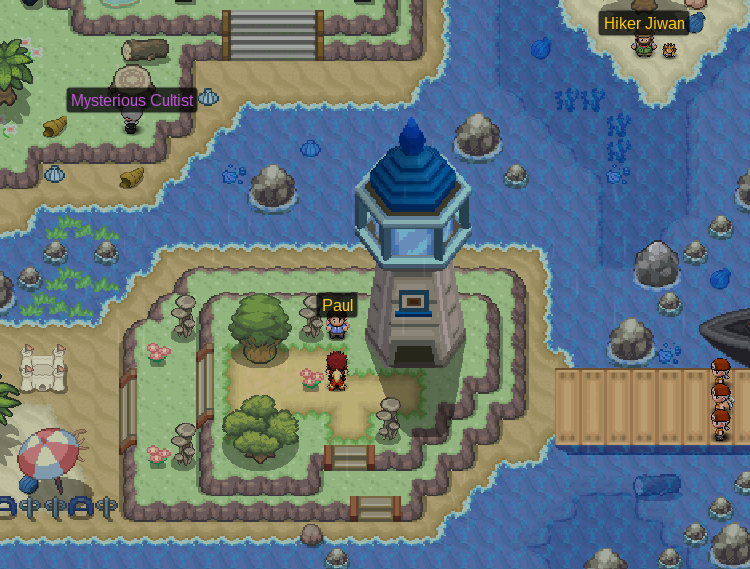
\includegraphics[width=\textwidth]{walkthrough/Sinnoh/paul-lilycove}

\section{Twinleaf Town}\label{sec:twinleaf-town}
Welcome to Sinnoh.
Go downstairs and talk with your grandma.

\section{Route 201}\label{sec:Route_201}
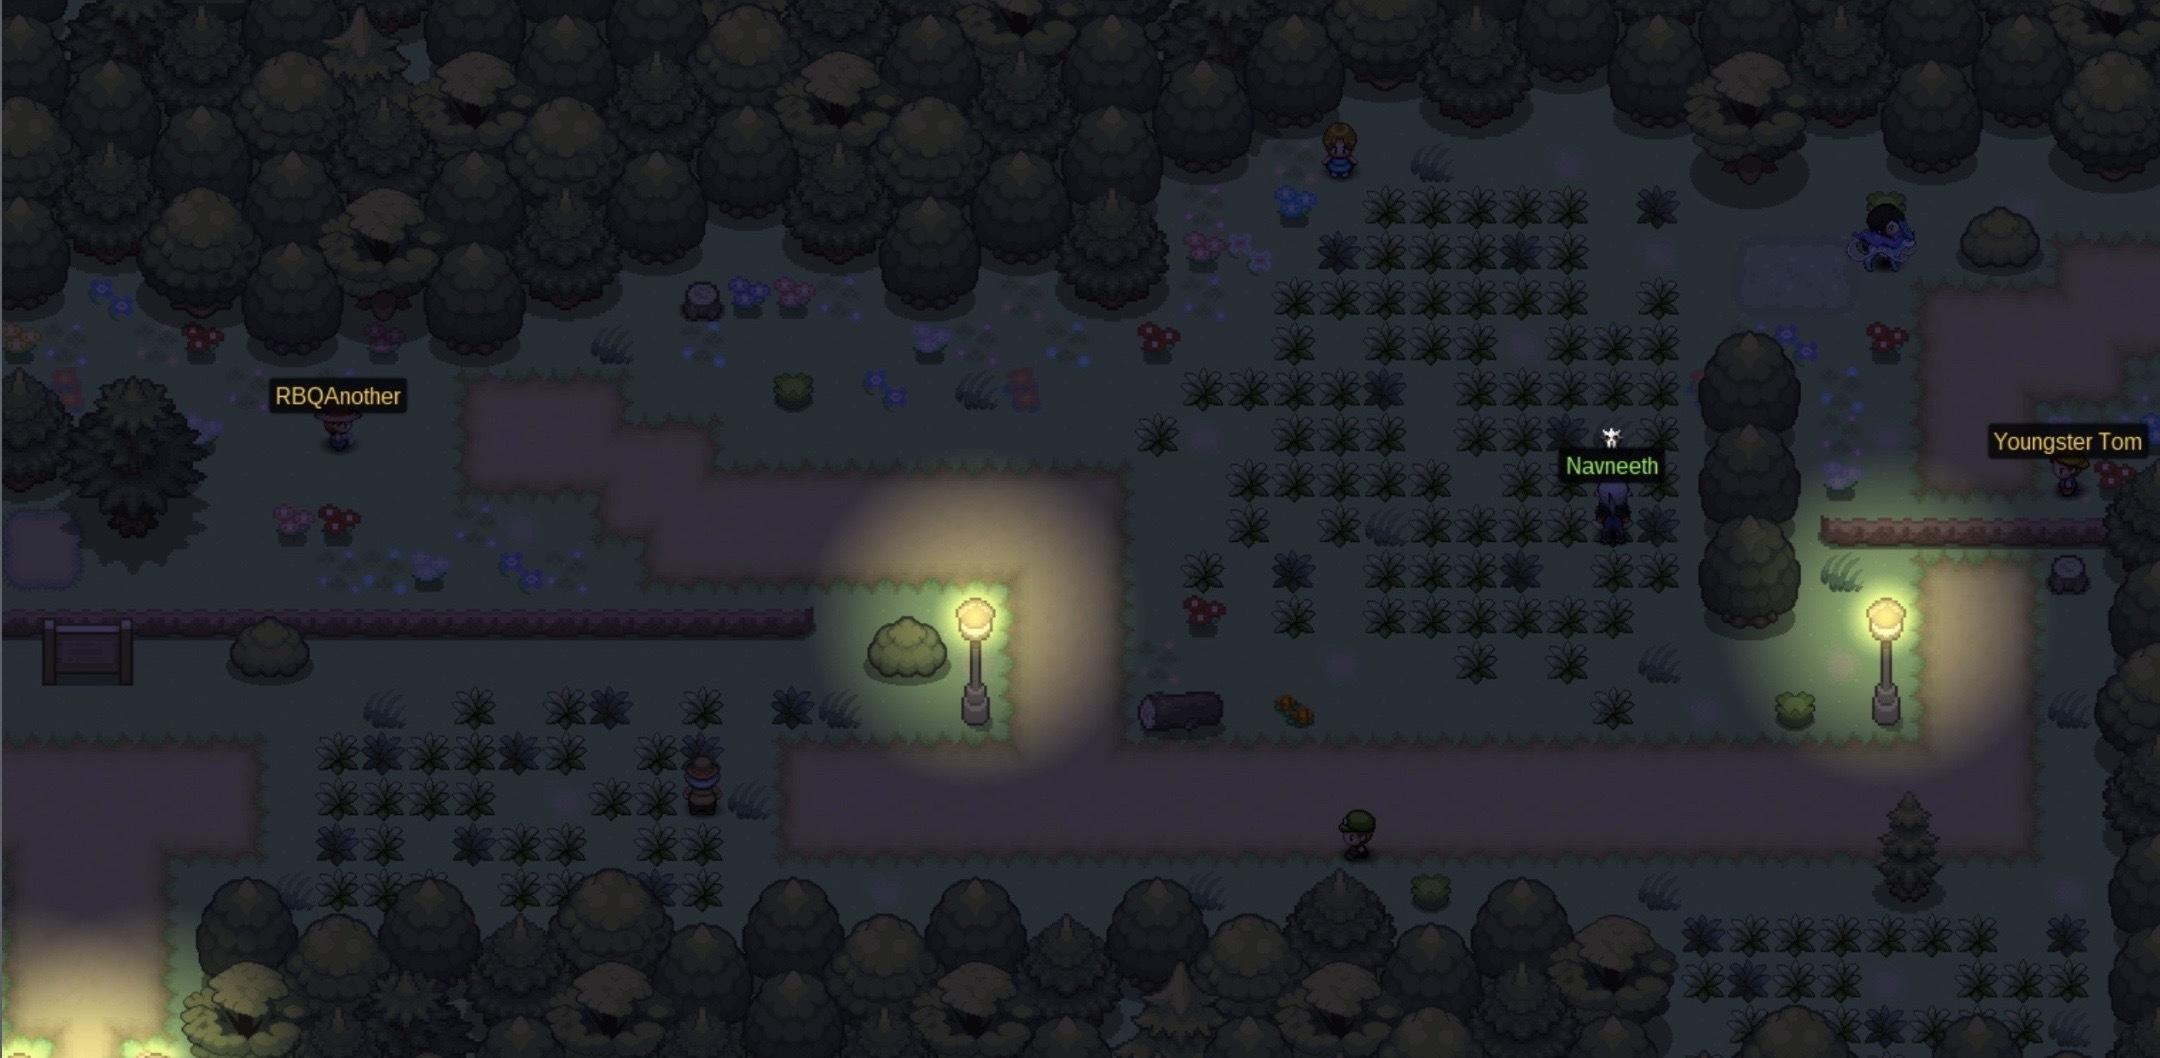
\includegraphics[width=\textwidth]{walkthrough/Sinnoh/Route_201}

Now we can go and visit Barry in his home, go up and talk with him
and then we can meet him in Route 201.
Prof  Rowan is going to stop us from walking in the grass without pokemon
and be ready to choose your starter.
Now go to the right and go to Prof Rowan lab.

\input{routes/Sinnoh/Route_201/Wild_Pokémon_(Land)}

\begin{mdframed}[style=PokemonSpotlight,nobreak=true,frametitle={Pokemon Spotlight: Bidoof}]
The humble Bidoof may not seem like an opposing foe, but some of them are \emph{Moody}.
The Hidden Ability \emph{Moody} raises one of the stats of the Pokémon with this
Ability by two stages (at random), then decreases another stat by one stage (at random).
A Bidoof or Bibarel that stays in battle long enough can reach maxed out stats
and become an unstoppable threat.

\begin{wrapfigure}{l}{0.33\textwidth}
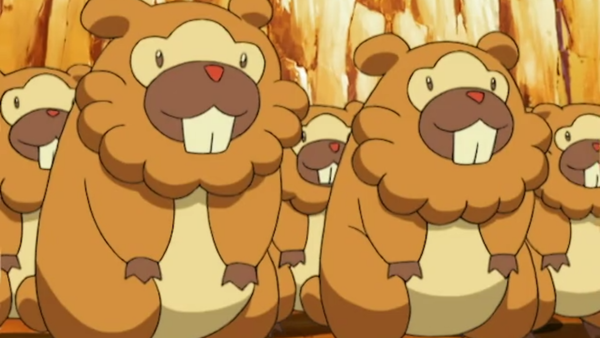
\includegraphics[width=0.33\textwidth]{walkthrough/Sinnoh/spotlight-bidoof}
\label{fig:spotlight-bidoof}
\end{wrapfigure}

The \emph{Moody} ability is perceived as so overpowered that Moody Bibarel has been
banned from most PvP formats.
Although \emph{Moody} will show up in only 5\% of Bidoofs, it may be worth the
grind in the early game to find one with this powerful ability, especially if
you do not pick Piplup as your starter.
The more common ability \emph{Simple} can also be utilized to double the effect of
\emph{Swords Dance} and make Bidoof/Bibarel a threatening foe.
Look for one with an Adamant nature and high IVs in Attack and Speed.
\end{mdframed}

\section{Lake Verity}\label{sec:Lake_Verity}

\input{routes/Sinnoh/Lake_Verity/Wild_Pokémon_(Land)}
\input{routes/Sinnoh/Lake_Verity/Wild_Pokémon_(Water)}

\section{Sandgem Town}\label{sec:sandgem-town}
Go to the Lab and we will find Barry. He will tell us that he is going to be at Jubilife School.
Enter the Lab and talk with Prof Rowan, But we already have everything from Prof Oak.

\subsection{Back to Grandma}\label{subsec:back-to-grandma}
After talking with Prof. Rowan we cant go to Route 202.
First we need to talk with our Grandma.
Go back to your house and talk with Grandma.
She will tell us that Barry's mom is worried, We need to visit her too.
Talk with his mother and she is going to ask us to tell Barry to go back home, he forgot something.

\section{Route 202}\label{sec:Route_202}
After talking with Grandma and Barry's mom, we can move on to Route 202.

\input{routes/Sinnoh/Route_202/Wild_Pokémon_(Land)}

\section{Jubilife City}\label{sec:jubilife-city}
Once in Jubilife city we need to find barry in the school.

\subsection{Student Locations}\label{subsec:student-locations}
Unfortunately, Barry is not there and we will have to help the teacher find her students first.

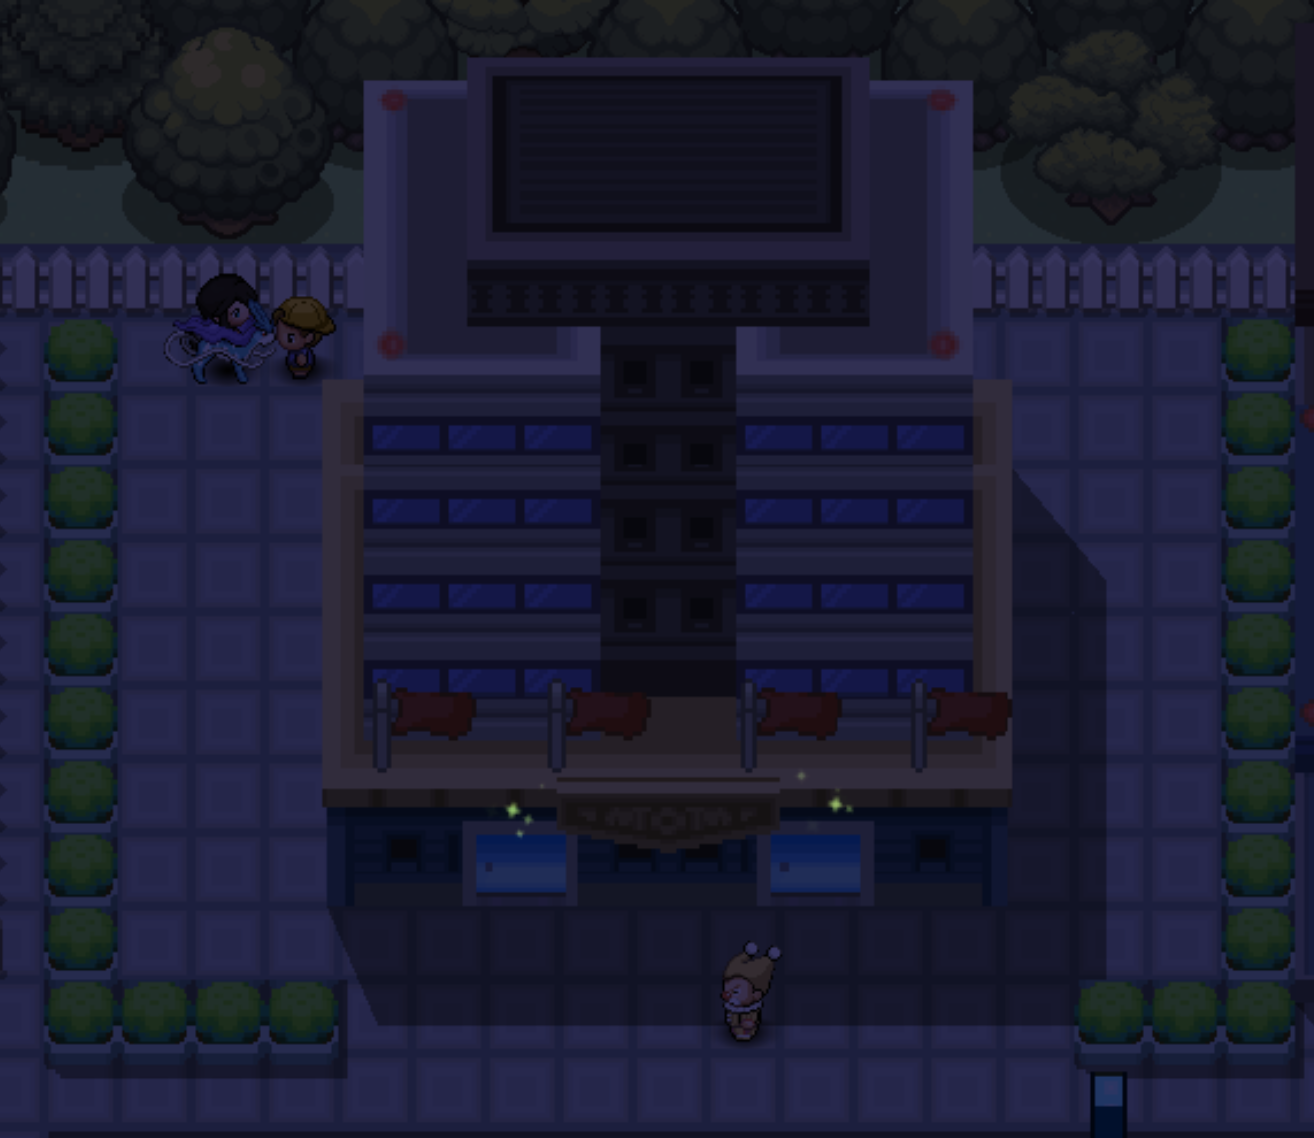
\includegraphics[width=0.5\textwidth]{walkthrough/Sinnoh/Jubilife-student-1}
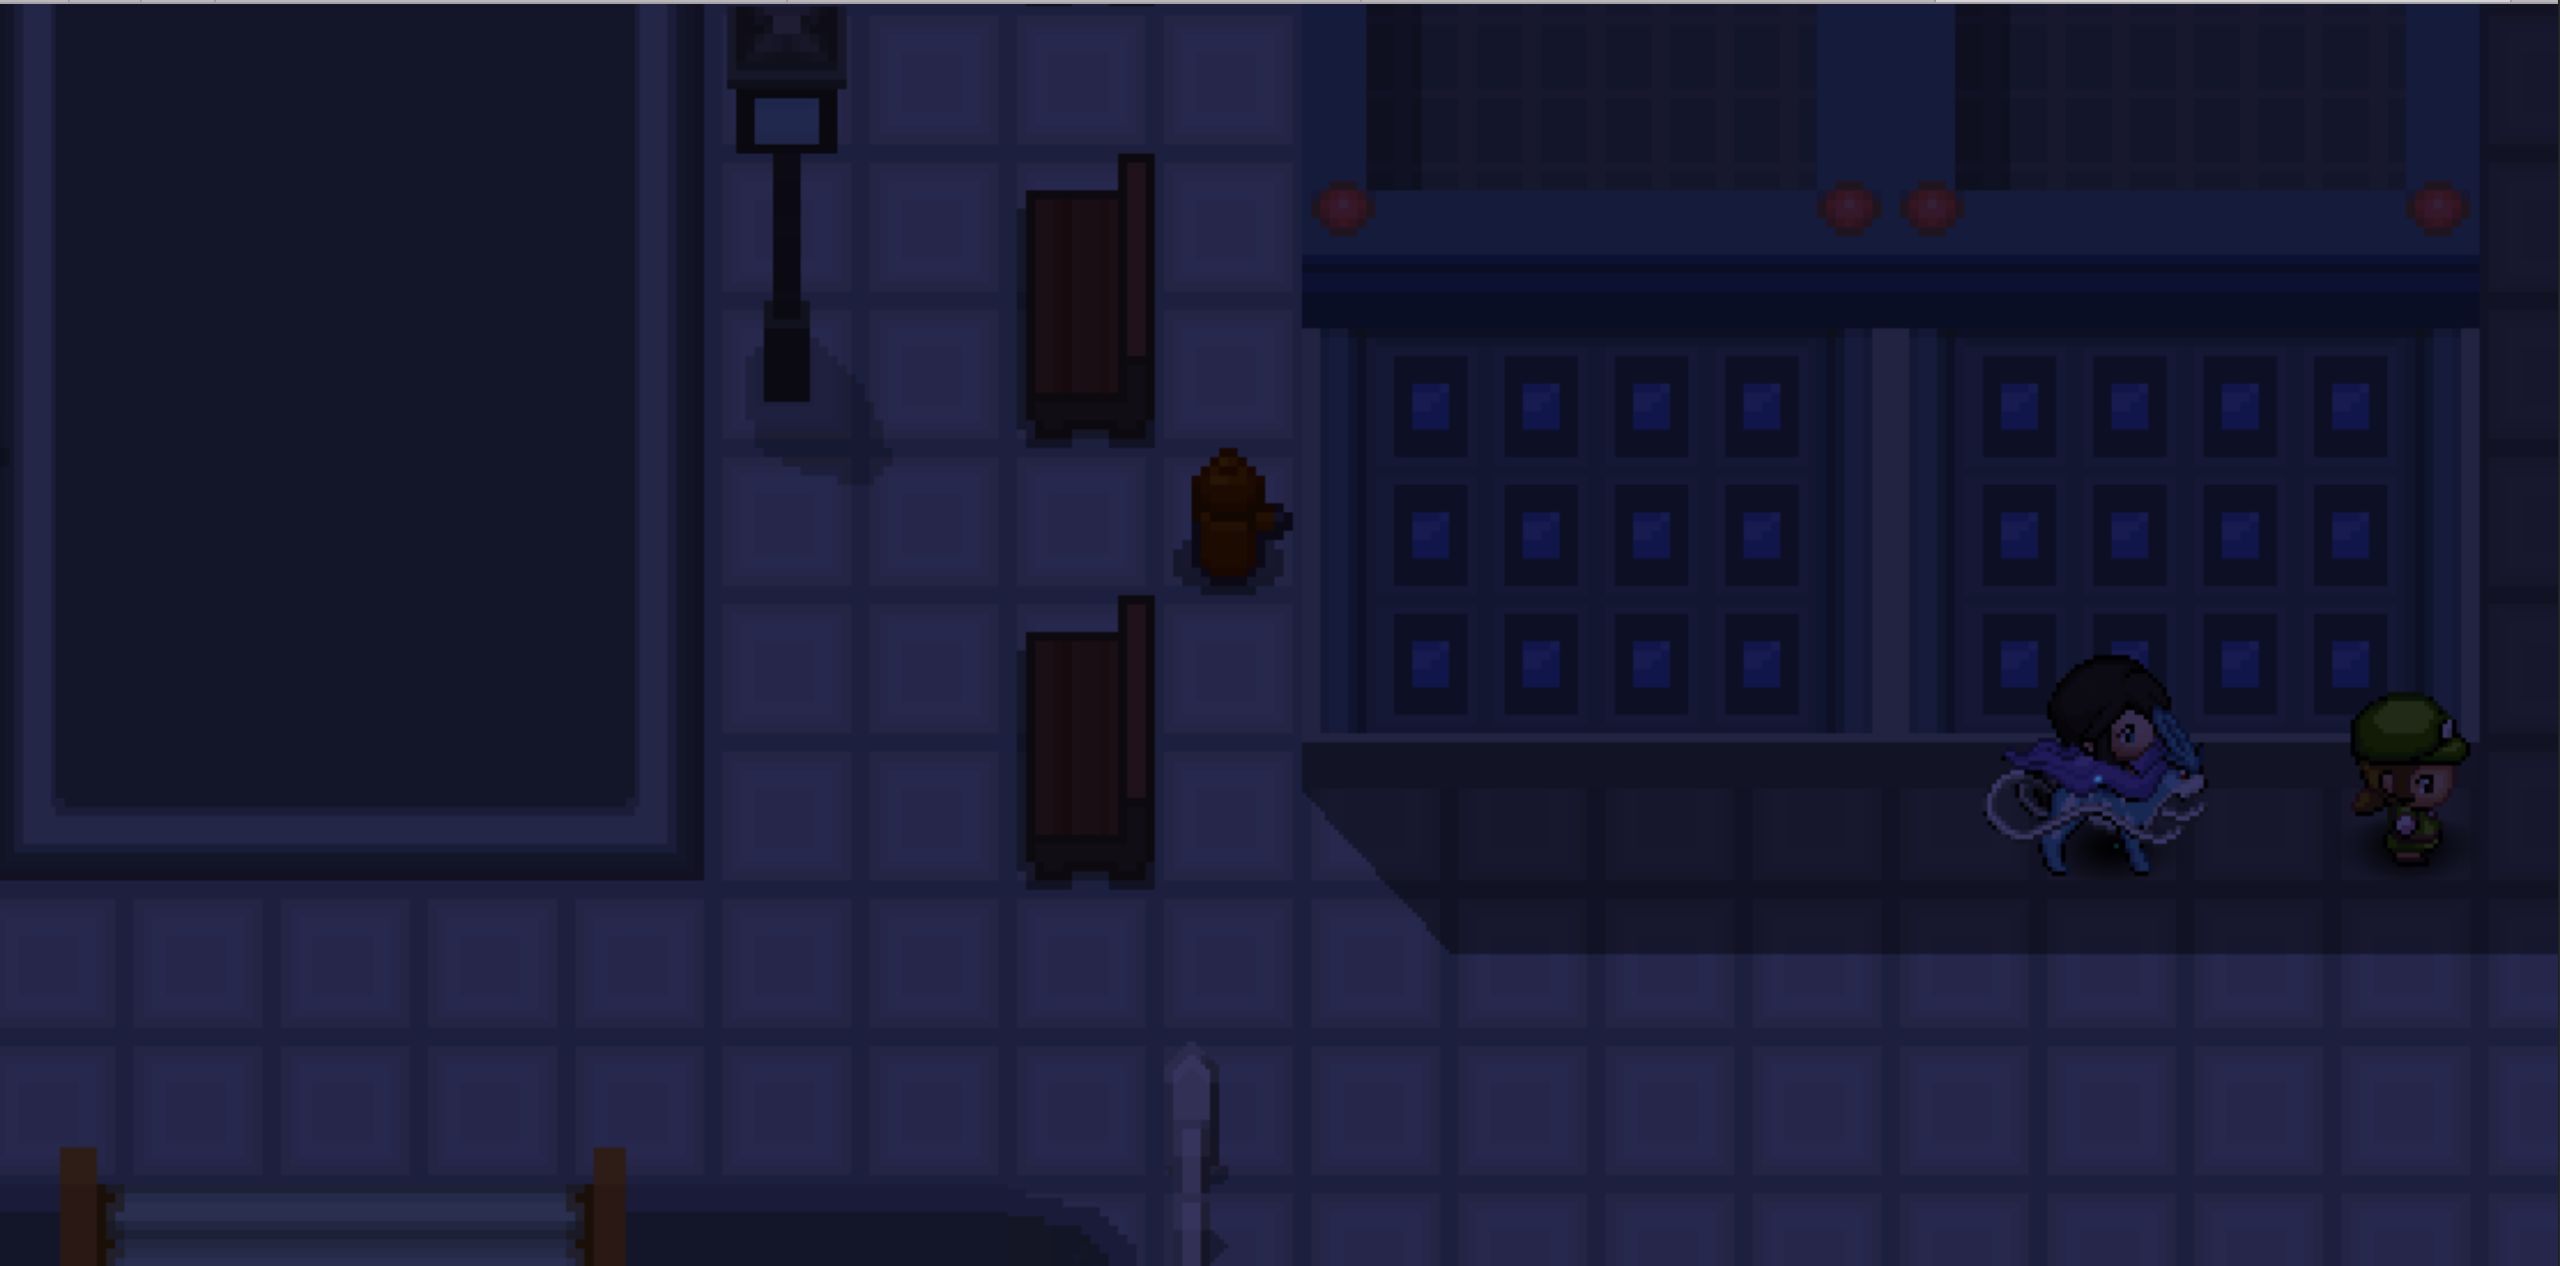
\includegraphics[width=0.5\textwidth]{walkthrough/Sinnoh/Jubilife-student-2}
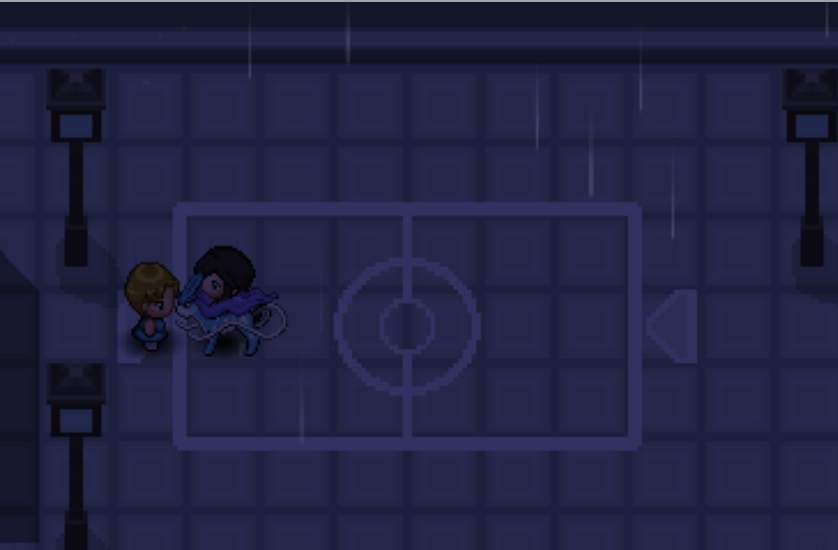
\includegraphics[width=0.5\textwidth]{walkthrough/Sinnoh/Jubilife-student-3}
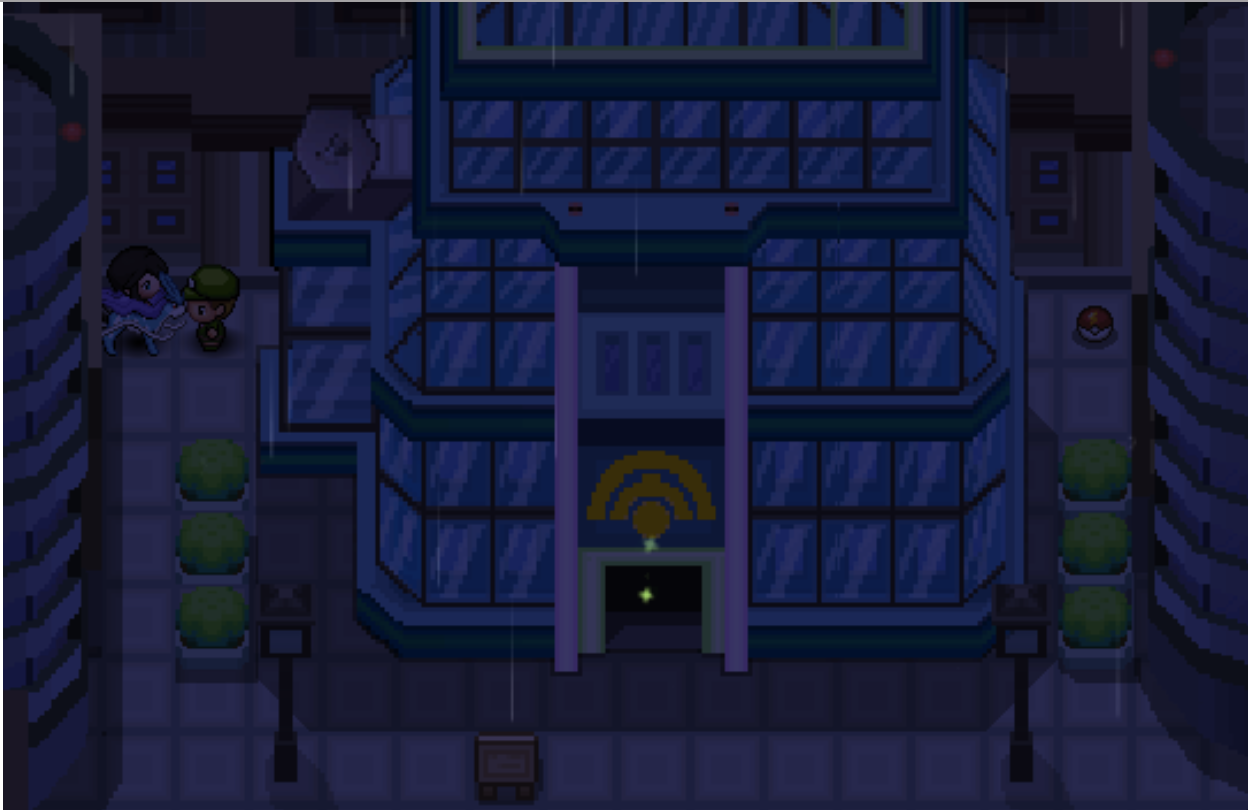
\includegraphics[width=0.5\textwidth]{walkthrough/Sinnoh/Jubilife-student-4}

And then go back to the school and talk with the Teacher.

\section{Route 218}\label{sec:Route_218}
Now we can find Barry at Route 218.
He will go back to his house and then we can go to Route 203.

\input{routes/Sinnoh/Route_218/Wild_Pokémon_(Land)}

\section{Route 203}\label{sec:Route_203}
Be ready to battle with Barry.
Beat him and enter the cave in the right.

\input{routes/Sinnoh/Route_203/Wild_Pokémon_(Land)}
\input{routes/Sinnoh/Route_203/Wild_Pokémon_(Water)}

\section{Oreburgh Gate}\label{sec:oreburgh-gate}
Ignore the upper route for now and go to the right.

\input{routes/Sinnoh/Oreburgh_Gate/Wild_Pokémon_(Oreburgh_Gate_1F)}

\section{Oreburgh City}\label{sec:oreburgh-city}
Now we are in the first city with a gym.
But first we need to Find Roark in the mine.

\subsection{Oreburgh Mine}\label{subsec:oreburgh-mine}

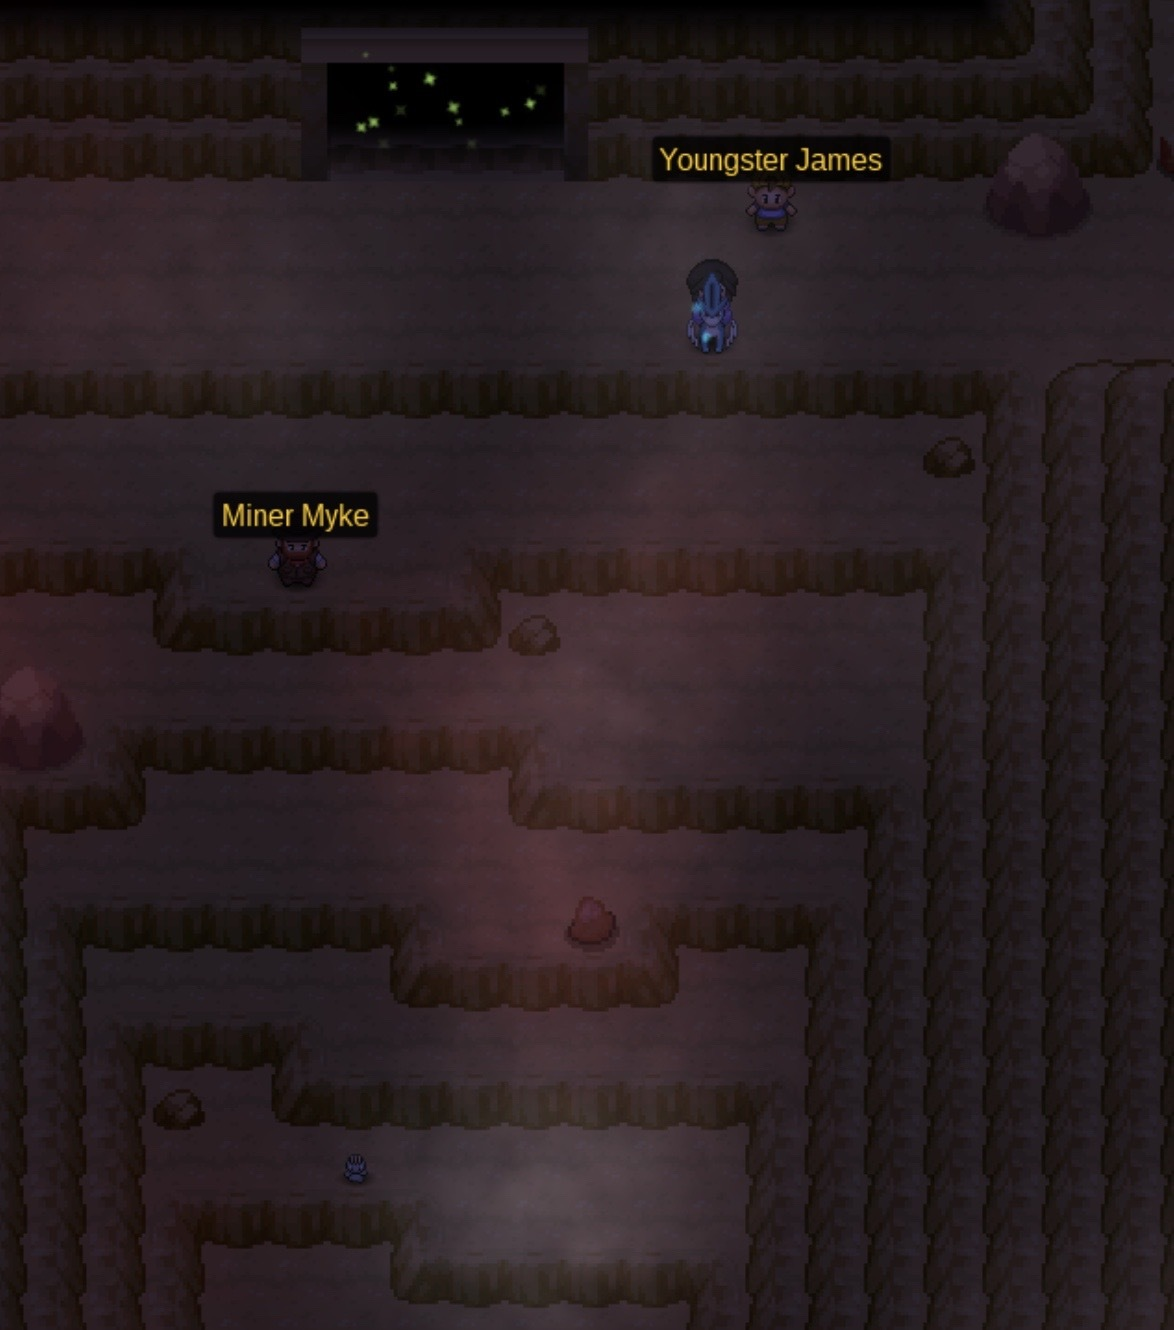
\includegraphics[width=\textwidth]{walkthrough/Sinnoh/oreburgh_mine}

Go all the way down to the mine and we are going to find him there,
talk with him and go back to the gym.

\input{routes/Sinnoh/Oreburgh_Mine/Wild_Pokémon_(Oreburgh_Mine_B1F)}
\input{routes/Sinnoh/Oreburgh_Mine/Wild_Pokémon_(Oreburgh_Mine_B2F_1R)}

\subsection{Oreburgh Gym}\label{subsec:oreburgh-gym}
Roark uses Rock-type pokemon.
After beating the gym go to Oreburgh City House 2 and you will find this NPC
selling rock smash, buy one we are going to need it later.

\section{Route 204}\label{sec:Route_204}
First head back to Jubilife City and talk with Looker and help him.
Now go to Route 204 and talk with the man in front of the cave enterence
in order to enter to the cave.

\input{routes/Sinnoh/Route_204/Wild_Pokémon_(Land)}
\input{routes/Sinnoh/Route_204/Wild_Pokémon_(Water)}

\section{Ravaged Path}\label{sec:Ravaged_Path}
This is why we needed to buy rock smash, smash the rock and go to the next area.

\input{routes/Sinnoh/Ravaged_Path/Wild_Pokémon_(Land)}
\input{routes/Sinnoh/Ravaged_Path/Wild_Pokémon_(Water)}

\section{Valley Windworks}\label{sec:valley-windworks}
Finally we are in Floaroma town but skip that town and go to route 205,
we are going to meet Sandy and we need to help her dad.
Go to the right and we are going to find Galactic Team again, Beat him.
Now we need a password to enter, Go back to Floaroma Town.

\input{routes/Sinnoh/Valley_Windworks/Wild_Pokémon_(Land)}
\input{routes/Sinnoh/Valley_Windworks/Wild_Pokémon_(Water)}

\section{Floaroma Town}\label{sec:floaroma-town}
Back in Floaroma Town, go to the top left area.
Beat the galactic guy and he is going to give us the password.
Go back to Valley Windworks and get ready to battle.

\section{Route 205}\label{sec:Route_205}
After you beat galactic guy, Go back to Route 205 and go to the north.
Nothing important in this route just a lot of trainers to get a lot of XP,
Go to the top and enter to Eterna Forest.

\input{routes/Sinnoh/Route_205/Wild_Pokémon_(Land)}
\input{routes/Sinnoh/Route_205/Wild_Pokémon_(Water)}

\section{Eterna Forest}\label{sec:Eterna_Forest}
Eterna forest have a lot of trainers as well.
After you beat them all go to the top right and you are in the second area of route 205.

\input{routes/Sinnoh/Eterna_Forest/Wild_Pokémon_(Land)}
\input{routes/Sinnoh/Eterna_Forest/Wild_Pokémon_(Headbuttable_Trees)}

\section{Eterna City}\label{sec:eterna-city}
Now we are in Eterna City.
Go to the gym and you are going to find Gardenia outside and she will ask you
if you can check the building in the north of the city.
Go to the building and we are going to find grunts for Galactic Team again.
Be ready to battle.
Once in the building go to the top and you will find
Commander Jupiter and Jevons, Talk with Jupiter and beat him.
After you beat him talk with Devons and help him to find some pokemon.
Pokemon Locations: TBD

After you find all pokemons, Talk with Jevons again and then go to the gym.

\subsection{Eterna City Gym}\label{subsec:eterna-city-gym}
Gardenia uses Grass-type Pokemon.
Beat her and get the badge.

\section{Route 211 (West)}\label{sec:Route_211_(West)}

\input{routes/Sinnoh/Route_211/Wild_Pokémon_(Land)}

\section{Mt. Coronet (Northern Area Part 1)}\label{sec:Mt._Coronet_North}
% \subsubsection{Wild Pokémon (Mt. Coronet North)}%
\label{ssubsec:WildPokmon(Mt.CoronetNorth)}%
\begin{longtable}{||l l l l l l l l||}%
\hline%
\rowcolor{gray}%
&Pokémon&Level Range&Morn&Day&Night&Held Item&Rarity Tier\\%
\hline%
\endhead%
\hline%
\rowcolor{gray}%

\includegraphics[width=0.02\textwidth]{pokemon/Cleffa}&Cleffa&13{-}17&Morn&Day&Night&Leppa Berry&\textcolor{RedOrange}{%
Rare%
}\\%
\hline%
\rowcolor{gray}%

\includegraphics[width=0.02\textwidth]{pokemon/Geodude}&Geodude&13{-}17&Morn&Day&Night&&\textcolor{black}{%
Common%
}\\%
\hline%
\rowcolor{gray}%

\includegraphics[width=0.02\textwidth]{pokemon/Gible}&Gible&5{-}14&Morn&&Night&&\textcolor{RedOrange}{%
Rare%
}\\%
\hline%
\rowcolor{gray}%

\includegraphics[width=0.02\textwidth]{pokemon/Machop}&Machop&13{-}17&Morn&Day&Night&&\textcolor{black}{%
Common%
}\\%
\hline%
\rowcolor{gray}%

\includegraphics[width=0.02\textwidth]{pokemon/Zubat}&Zubat&13{-}17&Morn&Day&Night&&\textcolor{black}{%
Common%
}\\%
\hline%
\end{longtable}%
\caption{Wild Pokemon in Mt. Coronet North (Mt. Coronet North)}

\section{Old Chateau}\label{sec:Old_Chateau}

\input{routes/Sinnoh/Old_Chateau/Wild_Pokémon_(Old_Chateau_1F)}

\section{Route 206}\label{sec:Route_206}
Nothing important in this routes just beat all the trainers to get Xp.

\section{Wayward Cave}\label{sec:Wayward_Cave}

\input{routes/Sinnoh/Wayward_Cave/Wild_Pokémon_(Wayward_Cave)}

\section{Route 207}\label{sec:Route_207}
In the cave from route 207 you will find Cyrus but you are not going to have a battle.

\input{routes/Sinnoh/Route_207/Wild_Pokémon_(Land)}

\begin{mdframed}[style=MyFrame,nobreak=true,frametitle={Pokemon Spotlight: Gligar}]

\begin{wrapfigure}{l}{0.33\textwidth}
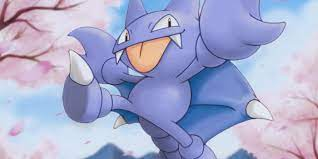
\includegraphics[width=0.33\textwidth]{walkthrough/Sinnoh/spotlight-gligar}
\label{fig:spotlight-gligar}
\end{wrapfigure}

Gligar's Hidden Ability, Poison Heal, allows it to be immune to status effects
when poisoned while also providing it with passive recovery, which is useful
alongside reliable recovery in Roost.
Using a Toxic Orb allows the poison to be applied automatically.

Gligar evolves into Gliscor when leveled up holding a Razor Fang during the night.
Find one with a Careful nature with high IVs in HP, Special Defense, and Speed.

If you don't want to grind for a Gligar with Poison Heal, a viable build can
also be made using Hyper Cutter.
Jolly or Impish Nature can also work.

\end{mdframed}

\section{Mt. Coronet South}\label{sec:mt.-coronet-south}
TODO

\section{Route 208}\label{sec:Route_208}

\subsection{Notables}\label{subsec:notables-route-208}

\begin{itemize}
    \item 2x Rawst Berry
    \item Pecha Berry
\end{itemize}

\input{routes/Sinnoh/Route_208/Wild_Pokémon_(Land)}
\input{routes/Sinnoh/Route_208/Wild_Pokémon_(Water)}
\input{routes/Sinnoh/Route_208/Wild_Pokémon_(Headbuttable_Trees)}

\section{Hearthome City}\label{sec:hearthome-city}
Now we are in Hearthome but the Gym is not available to us yet.
Proceed along to the right and find Barry, Be ready to battle.

\subsection{Notables}\label{subsec:notables-hearthome}

\begin{itemize}
    \item Caught Date Checker
    \item Move Relearner
    \item Move Tutor: Role Play
    \item TM Seller: Curse
\end{itemize}

\subsection{Amity Square}\label{subsec:amity-square}

\input{routes/Sinnoh/Amity_Square/Wild_Pokémon_(Land)}
\input{routes/Sinnoh/Amity_Square/Wild_Pokémon_(Water)}

\section{Route 209}\label{sec:Route_209}

\subsection{Notables}\label{subsec:notables-route-209}

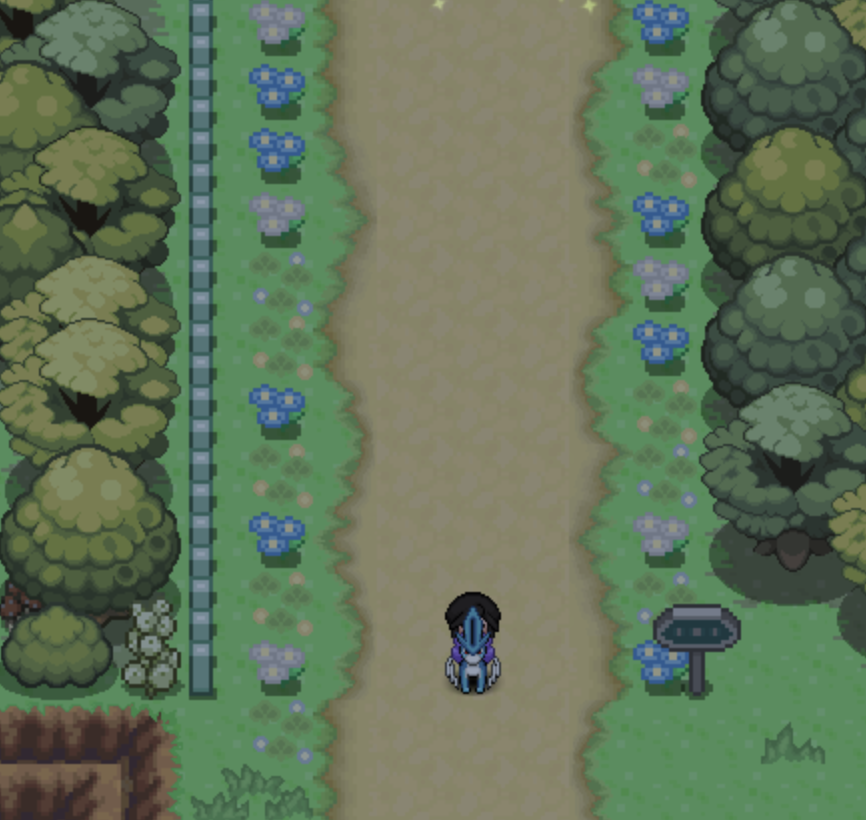
\includegraphics[width=\textwidth]{walkthrough/Sinnoh/Route_209}

Nothing important in this routes just battle with trainers

\begin{itemize}
    \item 2x Leppa Berry
    \item 1x Something Else
    \item 5x Dig Spots
    \item 4x Lum Berry
\end{itemize}

\input{routes/Sinnoh/Route_209/Wild_Pokémon_(Land)}
\input{routes/Sinnoh/Route_209/Wild_Pokémon_(Headbuttable_Trees)}
% \input{routes/Sinnoh/Route_209/Wild_Pokémon_(Diggable_Patches)}

\begin{mdframed}[style=MyFrame,nobreak=true,frametitle={Pokemon Spotlight: Chansey}]

Chansey's augmented physical bulk with Eviolite allows it to take powerful physical hits,
making it a staple on defensively oriented teams.
Wish and Natural Cure allow Chansey to heal its teammates and absorb status for them,
while access to Seismic Toss and Toxic helps prevent it from being setup bait.

\begin{wrapfigure}{l}{0.33\textwidth}
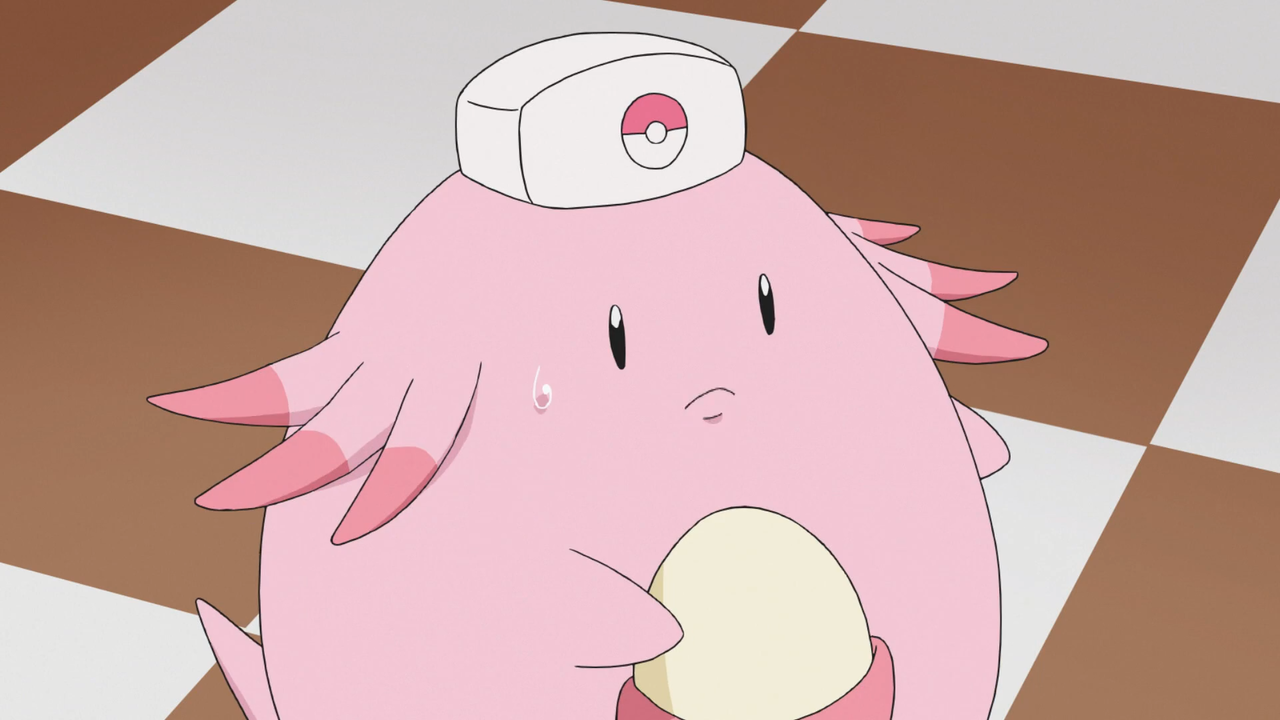
\includegraphics[width=0.33\textwidth]{walkthrough/Sinnoh/spotlight-chansey}
\label{fig:spotlight-chansey}
\end{wrapfigure}

Even with two ways of dealing damage, Chansey is still very passive and reliant on
Eviolite, and because of this it is largely shut down by Taunt or Knock Off.
Find one with a Bold nature with high IVs in Defense and Special Defense.

\end{mdframed}

\section{Lost Tower}\label{sec:Lost_Tower}

Lost Tower is a Sinnoh tower located in the north of Route 209.
There isn’t anything interesting in the tower however,
making it a side area for catching Pokémons and getting a couple items.
At the top of the tower the nice lady will give you a \emph{Spell Tag}.

\input{routes/Sinnoh/Lost_Tower/Wild_Pokémon_(Lost_Tower_1F)}
\input{routes/Sinnoh/Lost_Tower/Wild_Pokémon_(Lost_Tower_2F)}
\input{routes/Sinnoh/Lost_Tower/Wild_Pokémon_(Lost_Tower_3F)}
\input{routes/Sinnoh/Lost_Tower/Wild_Pokémon_(Lost_Tower_4F)}

\section{Route 210}\label{sec:Route_210}

\subsection{Notables}\label{subsec:notables-route-210}

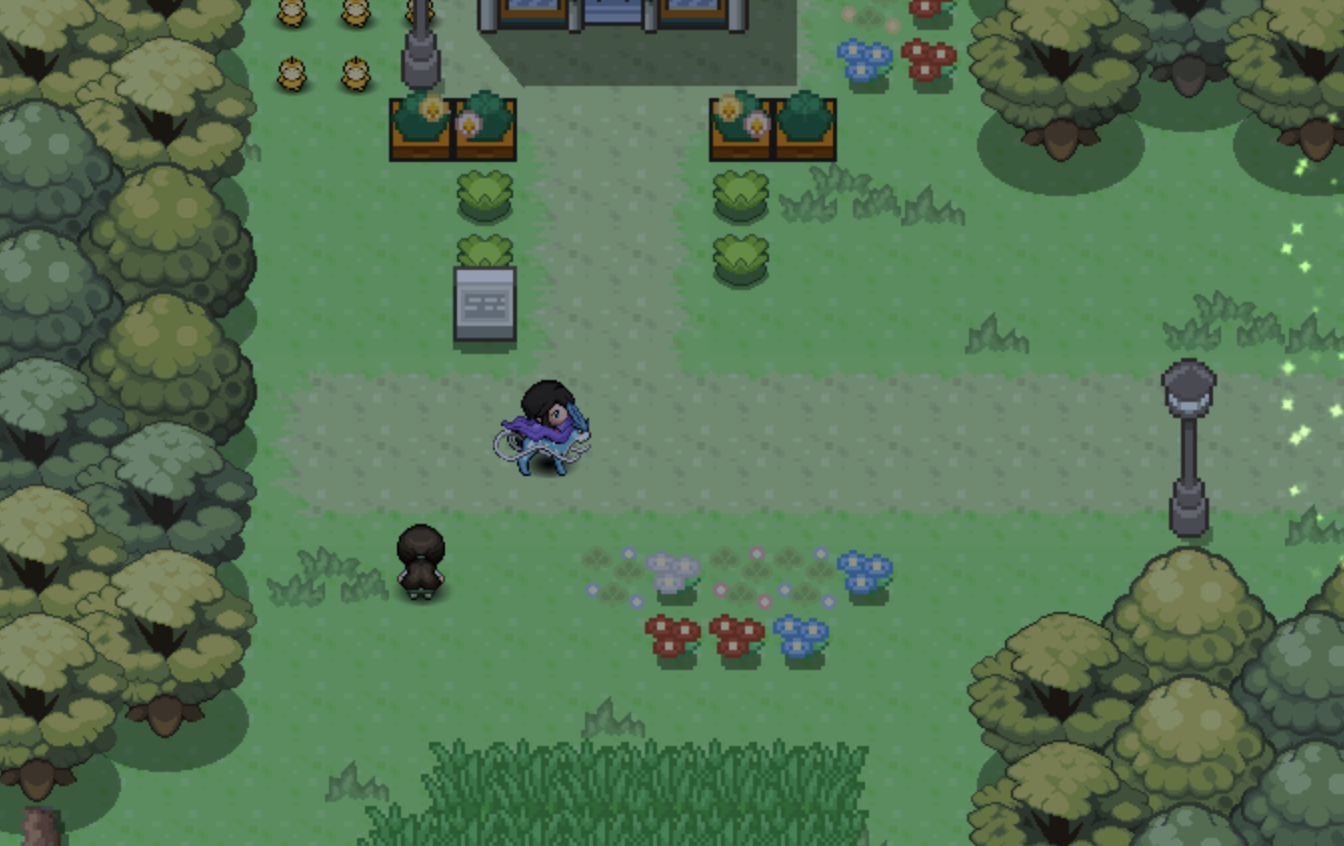
\includegraphics[width=\textwidth]{walkthrough/Sinnoh/Route_210}

\begin{itemize}
    \item 2x Leppa Berry
    \item 2x Lum Berry
\end{itemize}

\input{routes/Sinnoh/Route_210/Wild_Pokémon_(Land)}

\section{Solaceon Town}\label{sec:solaceon-town}

\subsection{Notables}\label{subsec:notables-solaceon-town}

\begin{itemize}
    \item 2x Sitrus Berry
    \item 2x Lum Berry
    \item News Reporter
    \item Daycare
\end{itemize}

\section{Route 215}\label{sec:Route_215}

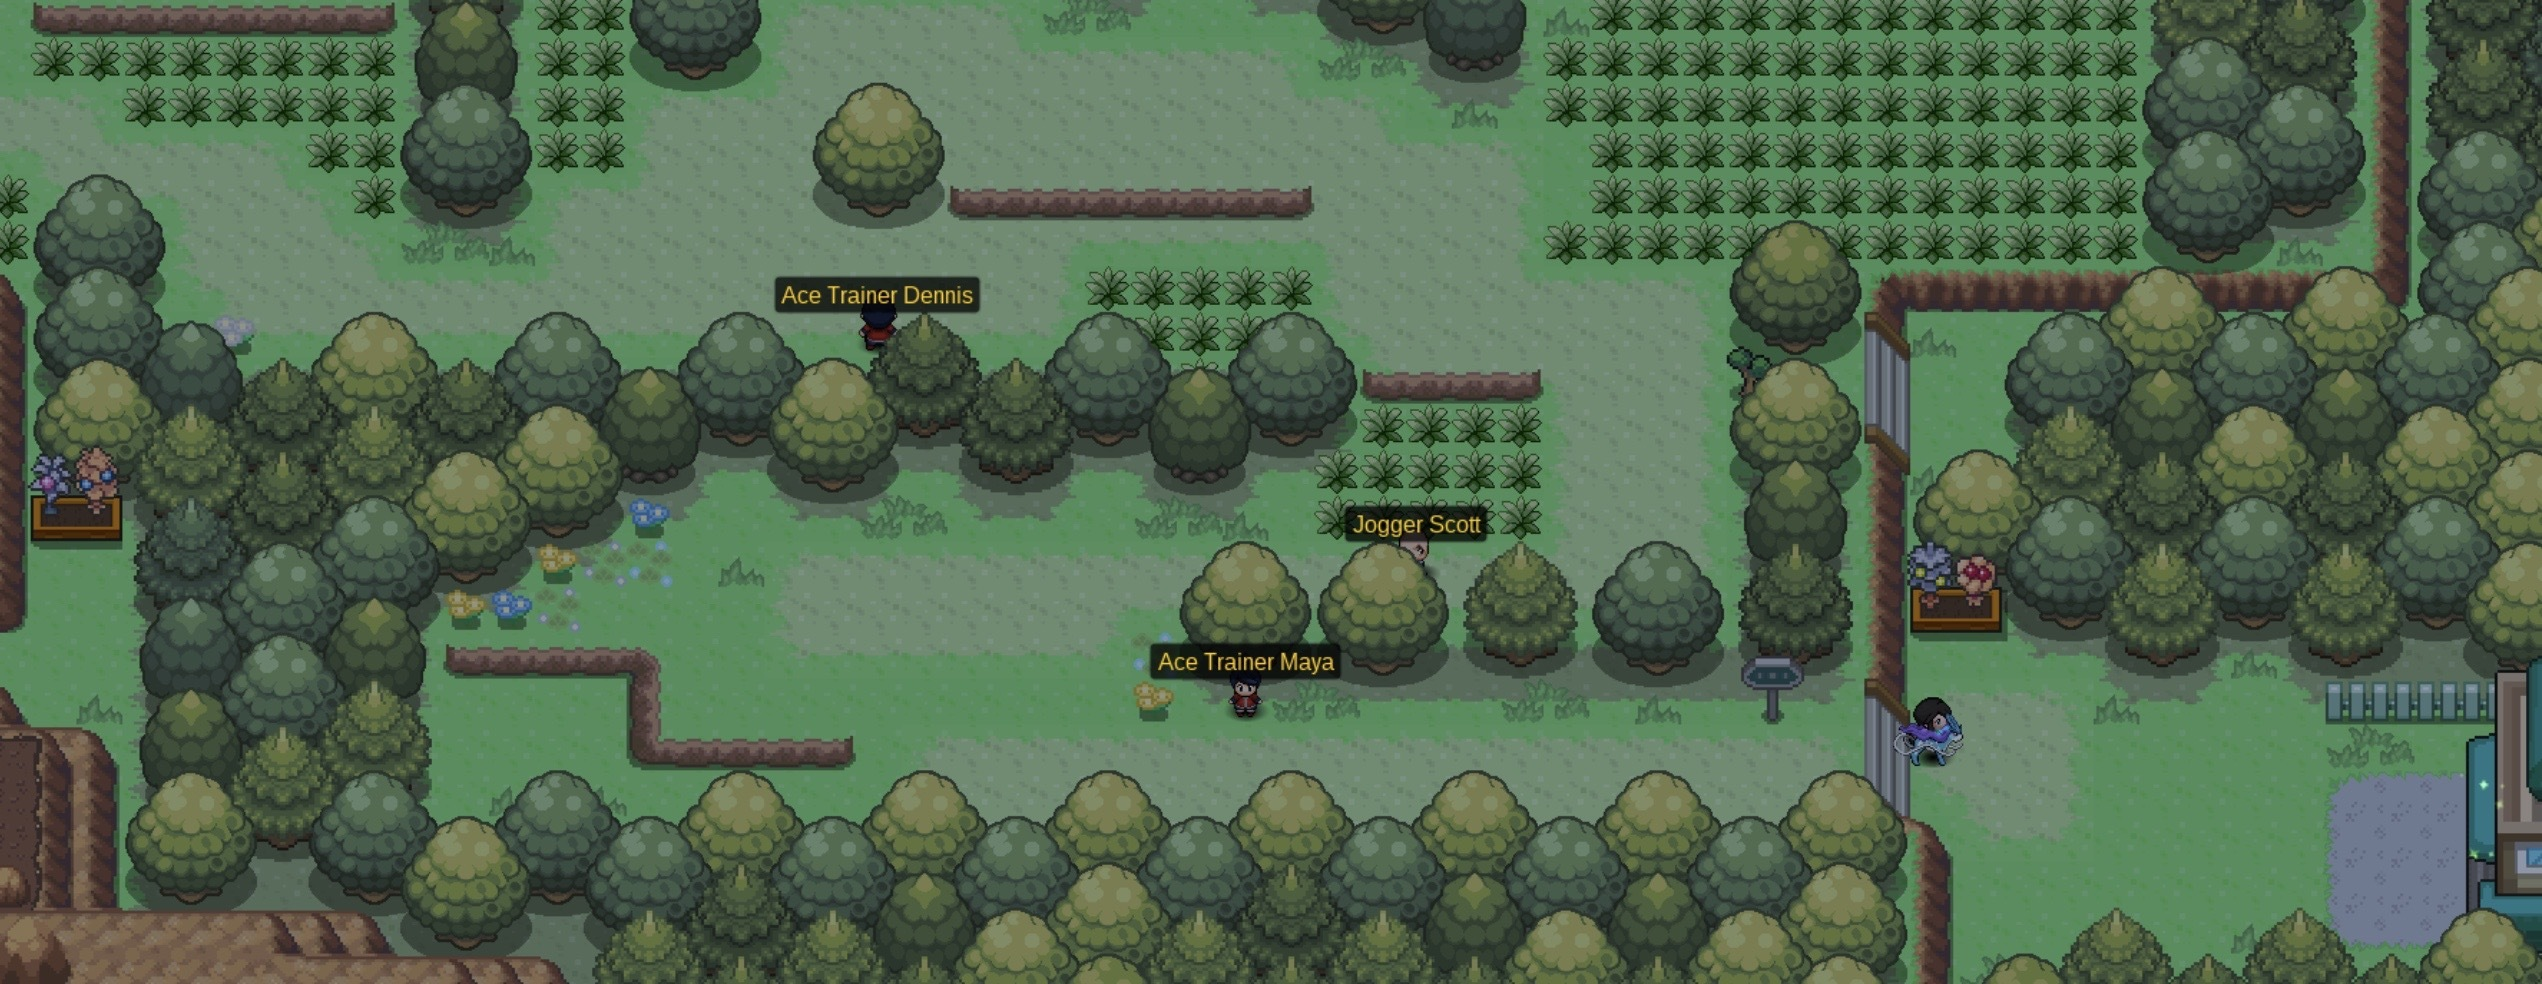
\includegraphics[width=\textwidth]{walkthrough/Sinnoh/Route_215}

\input{routes/Sinnoh/Route_215/Wild_Pokémon_(Land)}

\section{Veilstone City}\label{sec:veilstone-city}
Finally we are in the city.

Go to the gym and talk with dawn and then enter the gym.
In this gym we need to get two scrolls to be able to battle with the Leader.
Its always random so you need to battle with all trainers.
And be ready to battle with the leader.

\subsection{Veilstone City Gym}\label{subsec:veilstone-city-gym}
Maylene uses Fighting-type Pokemon.
Beat her and get the Cobble Badge.

\subsection{Dawn and After}\label{subsec:dawn-and-after}
Beat the gym and then you will find Dawn in the door.
She wil tell us that some grunts of the team galactic stole her pokedex and we need to help her.
Go to the north of the city and you will find Dawn with some Galactic Grunts.
Help her and be ready to battle.
After the battle, Talk with Dawn again and she will tell us to go to Pastoria City.

\section{Route 214}\label{sec:Route_214}

To go to Pastoria City you need to go to Route 214 in the south and follow all the routes.

\input{routes/Sinnoh/Route_214/Wild_Pokémon_(Land)}
\input{routes/Sinnoh/Route_214/Wild_Pokémon_(Water)}

\section{Route 213}\label{sec:Route_213}

\paragraph Valor Lakefront For now the Lake itself is blocked from access, so
we are quickly passing through the Lakefront as we continue through Route 213.

\input{routes/Sinnoh/Route_213/Wild_Pokémon_(Land)}
\input{routes/Sinnoh/Route_213/Wild_Pokémon_(Water)}

\section{Pastoria City}\label{sec:pastoria-city}
Go to the gym and get ready to battle with trainers and the leader.

\subsection{Pastoria City Gym}\label{subsec:pastoria-city-gym}
Wake uses Water-type Pokemon.
Beat him and you will get the Fen Badge and now you can use Surf.

\subsection{Notables}\label{subsec:notables-pastoria-city}

\begin{itemize}
    \item TM Tutor - Hone Claws \emph{(Requires Surf)}
\end{itemize}

\section{Cynthia and Cyrus}\label{sec:cynthia-and-cyrus}
After you beat the gym, Go to the north of Pastoria City
and you will find a Galatic Grunt there you need to follow him though routes 213
and Valor Lakefront you need to beat him.
Now go up and talk with Cynthia, She will ask us to give the medicine to the
Psyducks in Route 210 and Give Old Charm to her Grandma in Celestic Town.

\input{routes/Sinnoh/Valor_Lakefront/Wild_Pokémon_(Land)}

\section{Route 212 South}\label{sec:route-212-(south)}
We need to head to Route 210, so we might as well explore Route 212 on the way.
This area has plenty of trainers to work on.

\input{routes/Sinnoh/Route_212_South/Wild_Pokémon_(Land)}
\input{routes/Sinnoh/Route_212_South/Wild_Pokémon_(Water)}

\section{Route 212 North}\label{sec:route-212-north}
Plenty of trainers to level up on.
This area also contains the Pokemon Mansion.

\paragraph{Pokemon Mansion}
- Celeste will give you 5 Ultra Balls if you beat her.
- There is a Big Nugget in one of the rooms.
- There is a Rich Kid who will give you a Rare Candy for beating him.
- There are 3 Super Potions on the right side.

\input{routes/Sinnoh/Route_212_North/Wild_Pokémon_(Land)}
\input{routes/Sinnoh/Route_212_North/Wild_Pokémon_(Water)}

\section{Route 210 (North)}\label{sec:route-210-(north)}
Give the medicine to the Psyducks to access Route 210 North.

\section{Celestic Town}\label{sec:celestic-town}
In celestic Town we need to beat the Galatic Grunt blocking the cave.
After beating the Grunt, Cynthia's Grandma will appear behind you
and you need to give her the old charm.
Now enter in the cave and talk with this fossil, Cyrus will appear and be ready to the battle.

\subsection{Notables}\label{subsec:notables-celestic}

\begin{itemize}
    \item Move Tutor: Magic Room
    \item Move Tutor: Trick Room
    \item Move Tutor: Magic Coat
    \item Item Maniac
\end{itemize}

\section{Route 211 (East)}\label{sec:Route_211_(East)}
Before we head back to Hearthome City let's clear out some random trainers to
the west of Celestic Town.

\subsection{Notables}\label{subsec:notables-route-211-east}

\begin{itemize}
    \item 3x Dig Spots
\end{itemize}

% \input{routes/Sinnoh/Route_211/Wild_Pokémon_(Diggable_Patches)}

\section{Mt. Coronet (Center)}\label{sec:mt.-coronet-(center)}
Then enter Mt. Coronet (Center).
Just a couple of Trainers here we can fight.
Otherwise we are blocked by the Onix and Steelix.

\input{routes/Sinnoh/Mt._Coronet_North/Wild_Pokémon_(Mt._Coronet_Center)}

\section{Back to Hearthome City}\label{sec:back-to-hearthome-city}
TODO: Reorder this

From Celestic Town head east to Route 210 and then South through
Solaceon Town to Route 209.

\paragraph{Route 212}
Continue west to Hearthome City and then head south to Route 212
In Route 212 North, southwest of Pokemon mansion, surf west on the pond and
you can collect some Berries: Qualot and Hondew.
Continue South to Pastoria City.

\paragraph{Pastoria City}
You can now use Surf to reach the TM Tutor for Hone Claws.
Use Surf near the guy who stands at the middle of the city.
Surf east and stop surfing between two trees.
Head inside and you can find the item Mystic Water,
which boosts the power of the Water-type moves of a Pokémon that holds it.

\paragraph{Route 213}
Head east out of Pastoria City
Surf southeast from Fisherman Kenneth (the fisherman that fought you).
Head into the sea between two rocks.
There are a few Trainers for you to fight and some items for you to collect in that area.
- Big Pearl in bottom-right rock near Sailor Paul.
- Water Stone on a sandbar.

\paragraph{Route 214}
Keep going North through Valor Lakefront to Route 214.
In the northern area there is a small pond you can surf across to reach
a Max Potion.

\paragraph{Mt. Coronet (South)}
Head to the south.
Go up the stairs that leads to another pond.
Surf east, and you can get the Dawn Stone.
Upstairs you can find Rock Slide.
There is a Galactic Grunt protecting a passage way but you cannot access yet.

\begin{longtable}{|| l l l l ||}%
\hline%
&Dusk Stone&x 1&Not respawnable\\%
\multicolumn{4}{||m{\textwidth}||}{In the south-east corner of Mt. Coronet South. Requires Surf.}%
\hline%
&TM48 — Rock Slide&x 1&Not respawnable\\%
\multicolumn{4}{||m{\textwidth}||}{In the south-west corner of Mt. Coronet 2F.}%
\hline%
&Escape Rope&x 1&Not respawnable\\%
\multicolumn{4}{||m{\textwidth}||}{Near the north-west corner of Mt. Coronet 2F, next to the Rock Smash rocks.}%
\hline%
&Hyper Potion&x 2&Not respawnable\\%
\multicolumn{4}{||m{\textwidth}||}{In the north-east corner of the main part of Mt. Coronet 2F.}%
\hline%
&Star Piece&x 1&Not respawnable\\%
\multicolumn{4}{||m{\textwidth}||}{In the east-most room of Mt. Coronet 2F, accessible from the eastmost ladder of 3F.}%
\hline%
&Revive&x 1&Not respawnable\\%
\multicolumn{4}{||m{\textwidth}||}{Hidden item. On the rock adjacent to the stairs in Mt. Coronet 3F.}%
\hline%
\endhead%
\hline%
\caption{Items in Mt. Coronet South}%
\label{tab:Mt.CoronetSouthItems}%
\end{longtable}

\paragraph{Route 206}
The area under the biking road is now accessible via Surf.
There are a number of trainers to defeat here.
There is a Rare Candy to be obtained in the top left.

\input{routes/Sinnoh/Route_206/Wild_Pokémon_(Land)}

\paragraph{Wayward Cave}

Wayward Cave has the main visible entrance, and another secret entrance under
the bridge.
The secret entrance leads to TM Tutor Tri Attack.

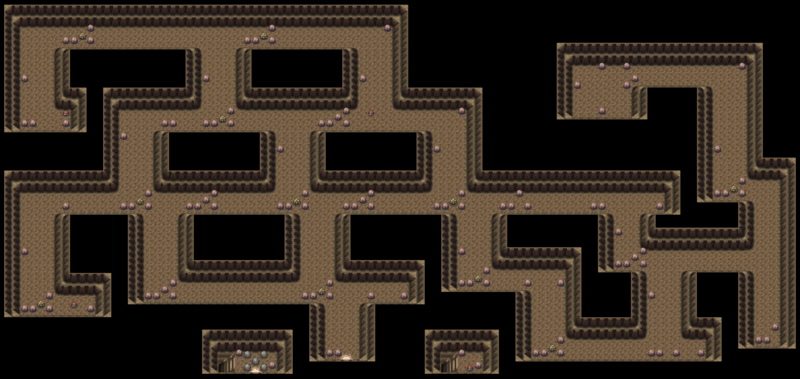
\includegraphics[width=\textwidth]{walkthrough/Sinnoh/wayward-cave}

\input{routes/Sinnoh/Wayward_Cave/Wild_Pokémon_(Wayward_Cave)}

\subsection{Hearthome City Gym}\label{subsec:hearthome-city-gym}
The Gym in Hearthome City is next to where you battled with Barry next to Route 209.
Once in Hearthome City go to the gym and be ready to battle.
This gym is a bit hard without Flash but you can catch a Roselia in Route 212
and it can learn Flash.
I made this tutorial to this gym maze.

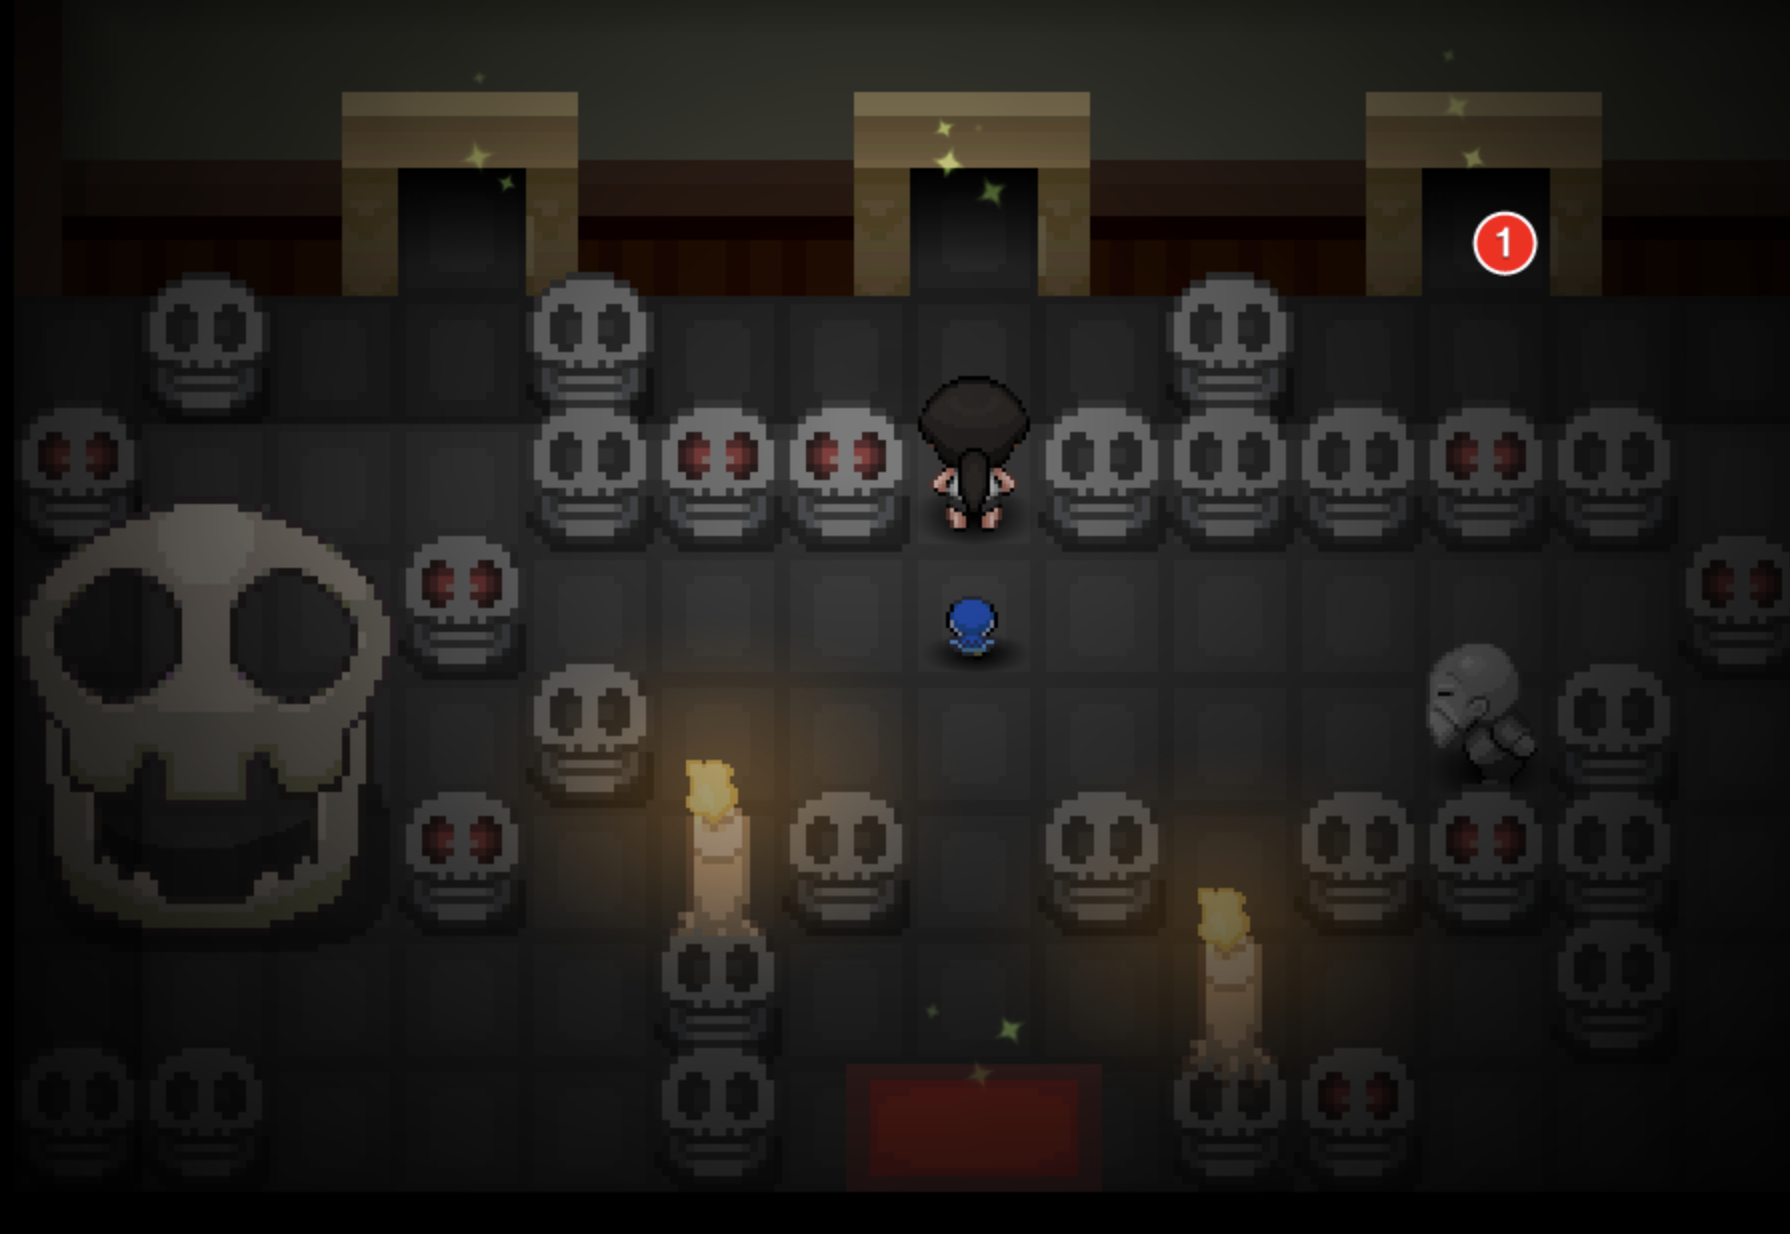
\includegraphics[width=\textwidth]{walkthrough/Sinnoh/hearthome_gym_1}
And the next part:

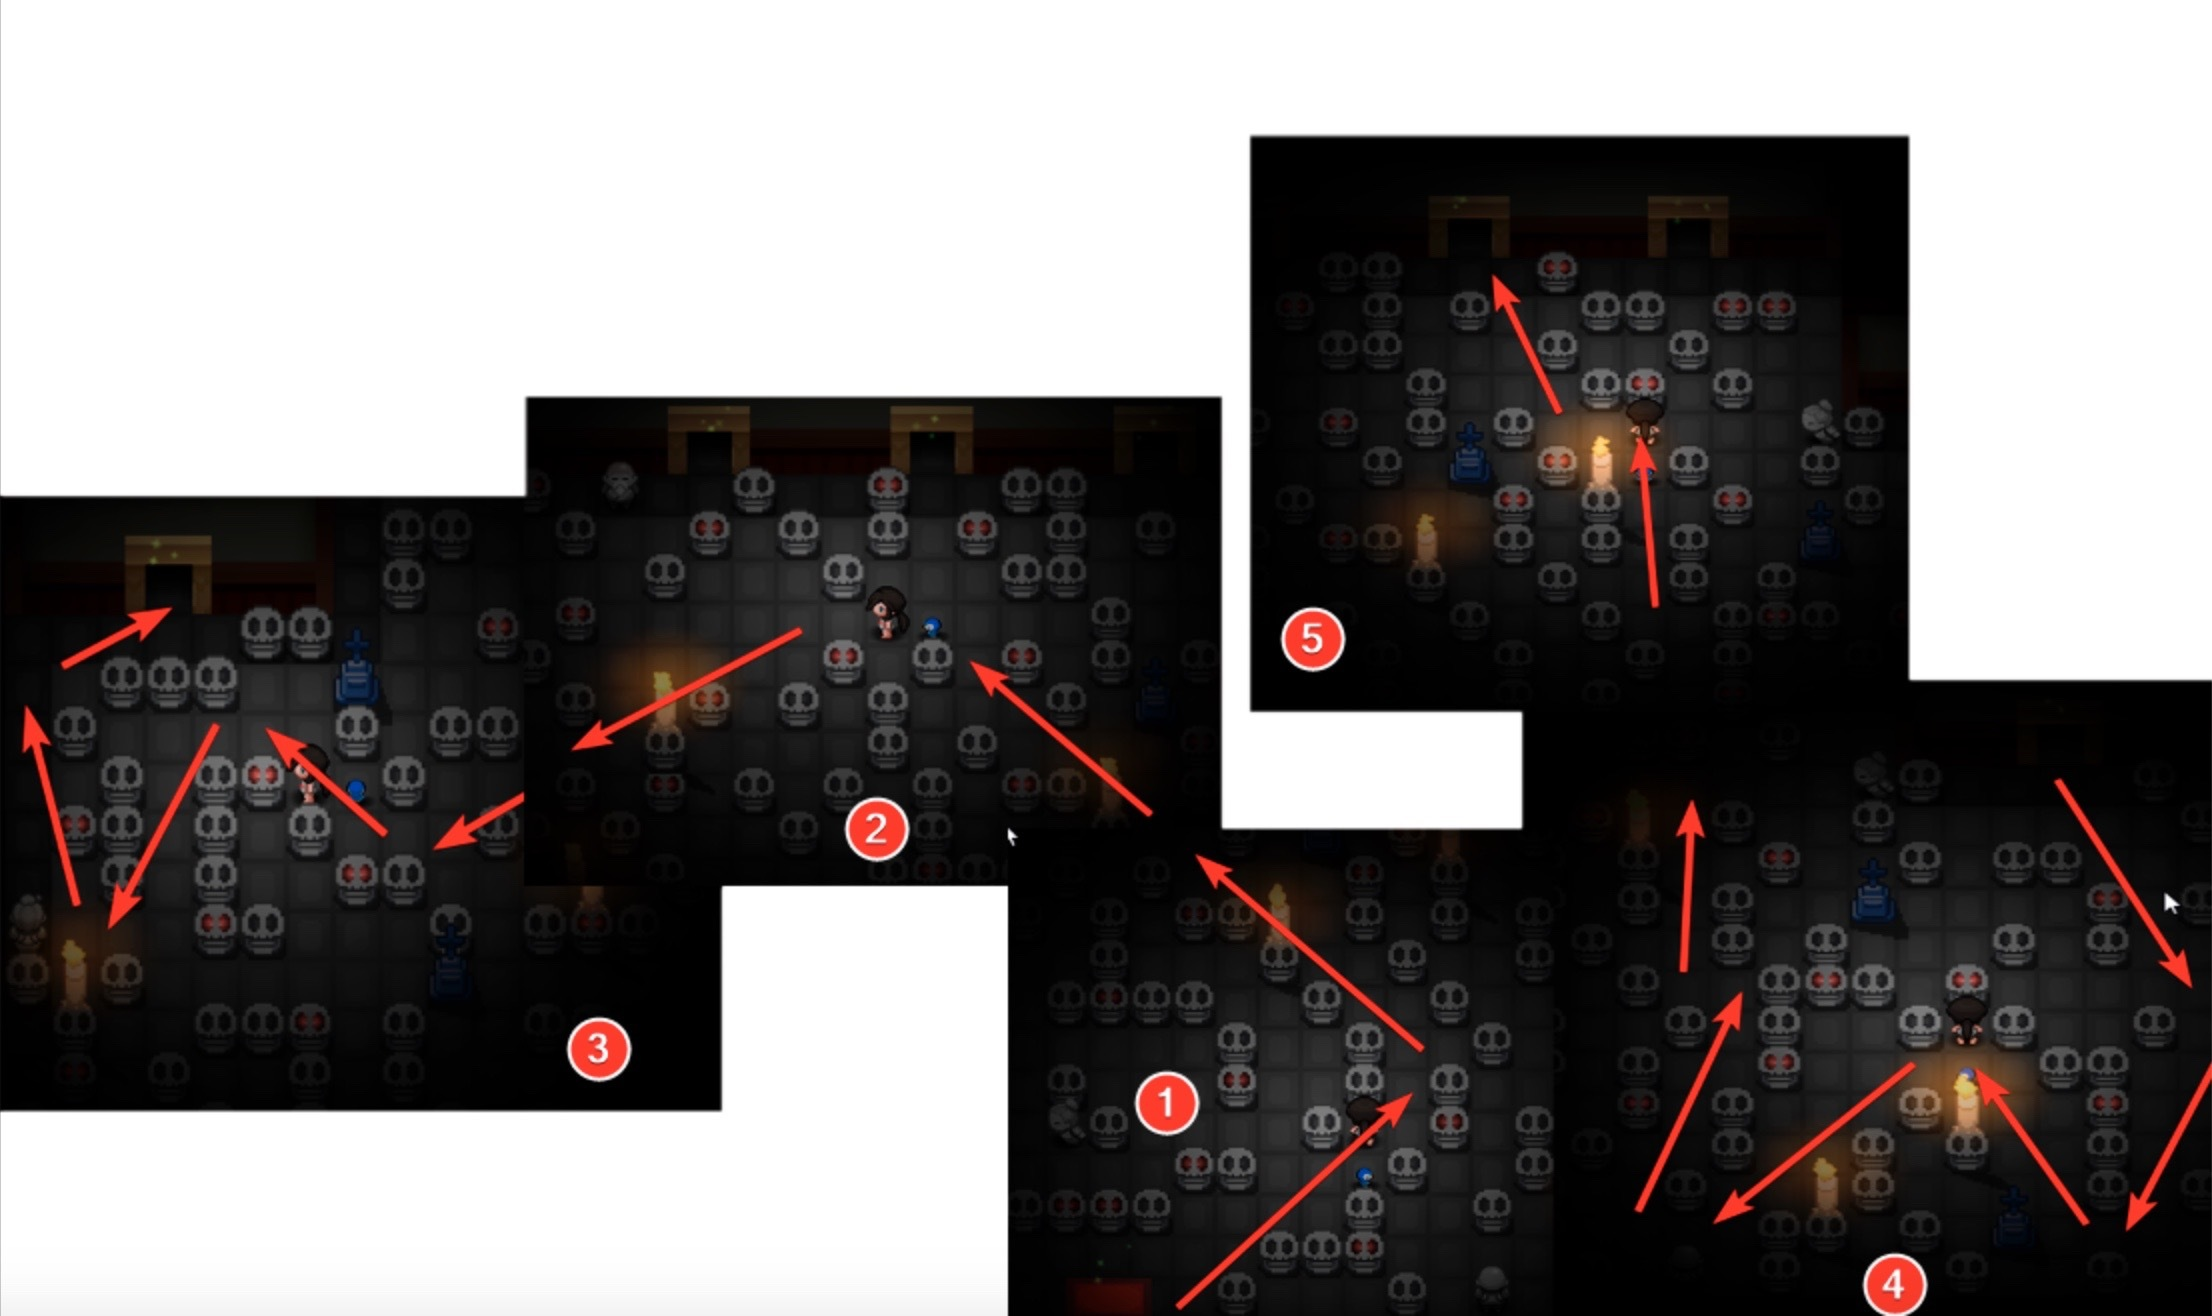
\includegraphics[width=\textwidth]{walkthrough/Sinnoh/hearthome_gym_2}
Fantina uses Ghost-type Pokemon.
Beat her and you will get the Relic Badge.
She will tell us to visit the Library in Canalave City.

\section{Fuego Ironworks}\label{sec:fuego-ironworks}
Go to Route 205.
Remember the house south of Eterna Forest,
which you can take a rest and heal your Pokémon?
Head south from there and go down the stairs.
Turn west when you can.
You will see a river.
Now that you can use Surf, you can get through this river.
Keep travelling north, and this river will bring you to Fuego Ironworks.
Travelling south brings you to Valley Windworks.
Go to the north of the river.
You will see a patch of grass.
Go through it, and you will see a factory.

here are many Trainers inside.
You will also see something familiar if you have played
Pokémon FireRed and LeafGreen.
Yes, these are the spinners again.
Step on it, and you will spin in circles and travel in the direction
that the arrow of the spinner points to.
For example, if you step on a spinner with an arrow on it that points to the left,
you will spin to the left and keep going until you hit something or another spinner.

There are a few Trainers for you to fight.
Fight them, collect the items and use the spinners to go around.
Eventually you will reach the boiler and Mr. Fuego.
He will give you a Fire Stone.
Afterwards, collect TM35 (Flamethrower), and leave Fuego Ironworks.

There is an one-way exit east of Fuego Ironworks, which leads you back to Route 205.
Jump down the two ledges, and you will find yourself near the entrance of
Eterna Forest and the healing house.

\section{Back to Jubilife City}\label{sec:back-to-jubilife-city}
Time to travel back to Jubilife City, by way of Route 208 to Route 218.

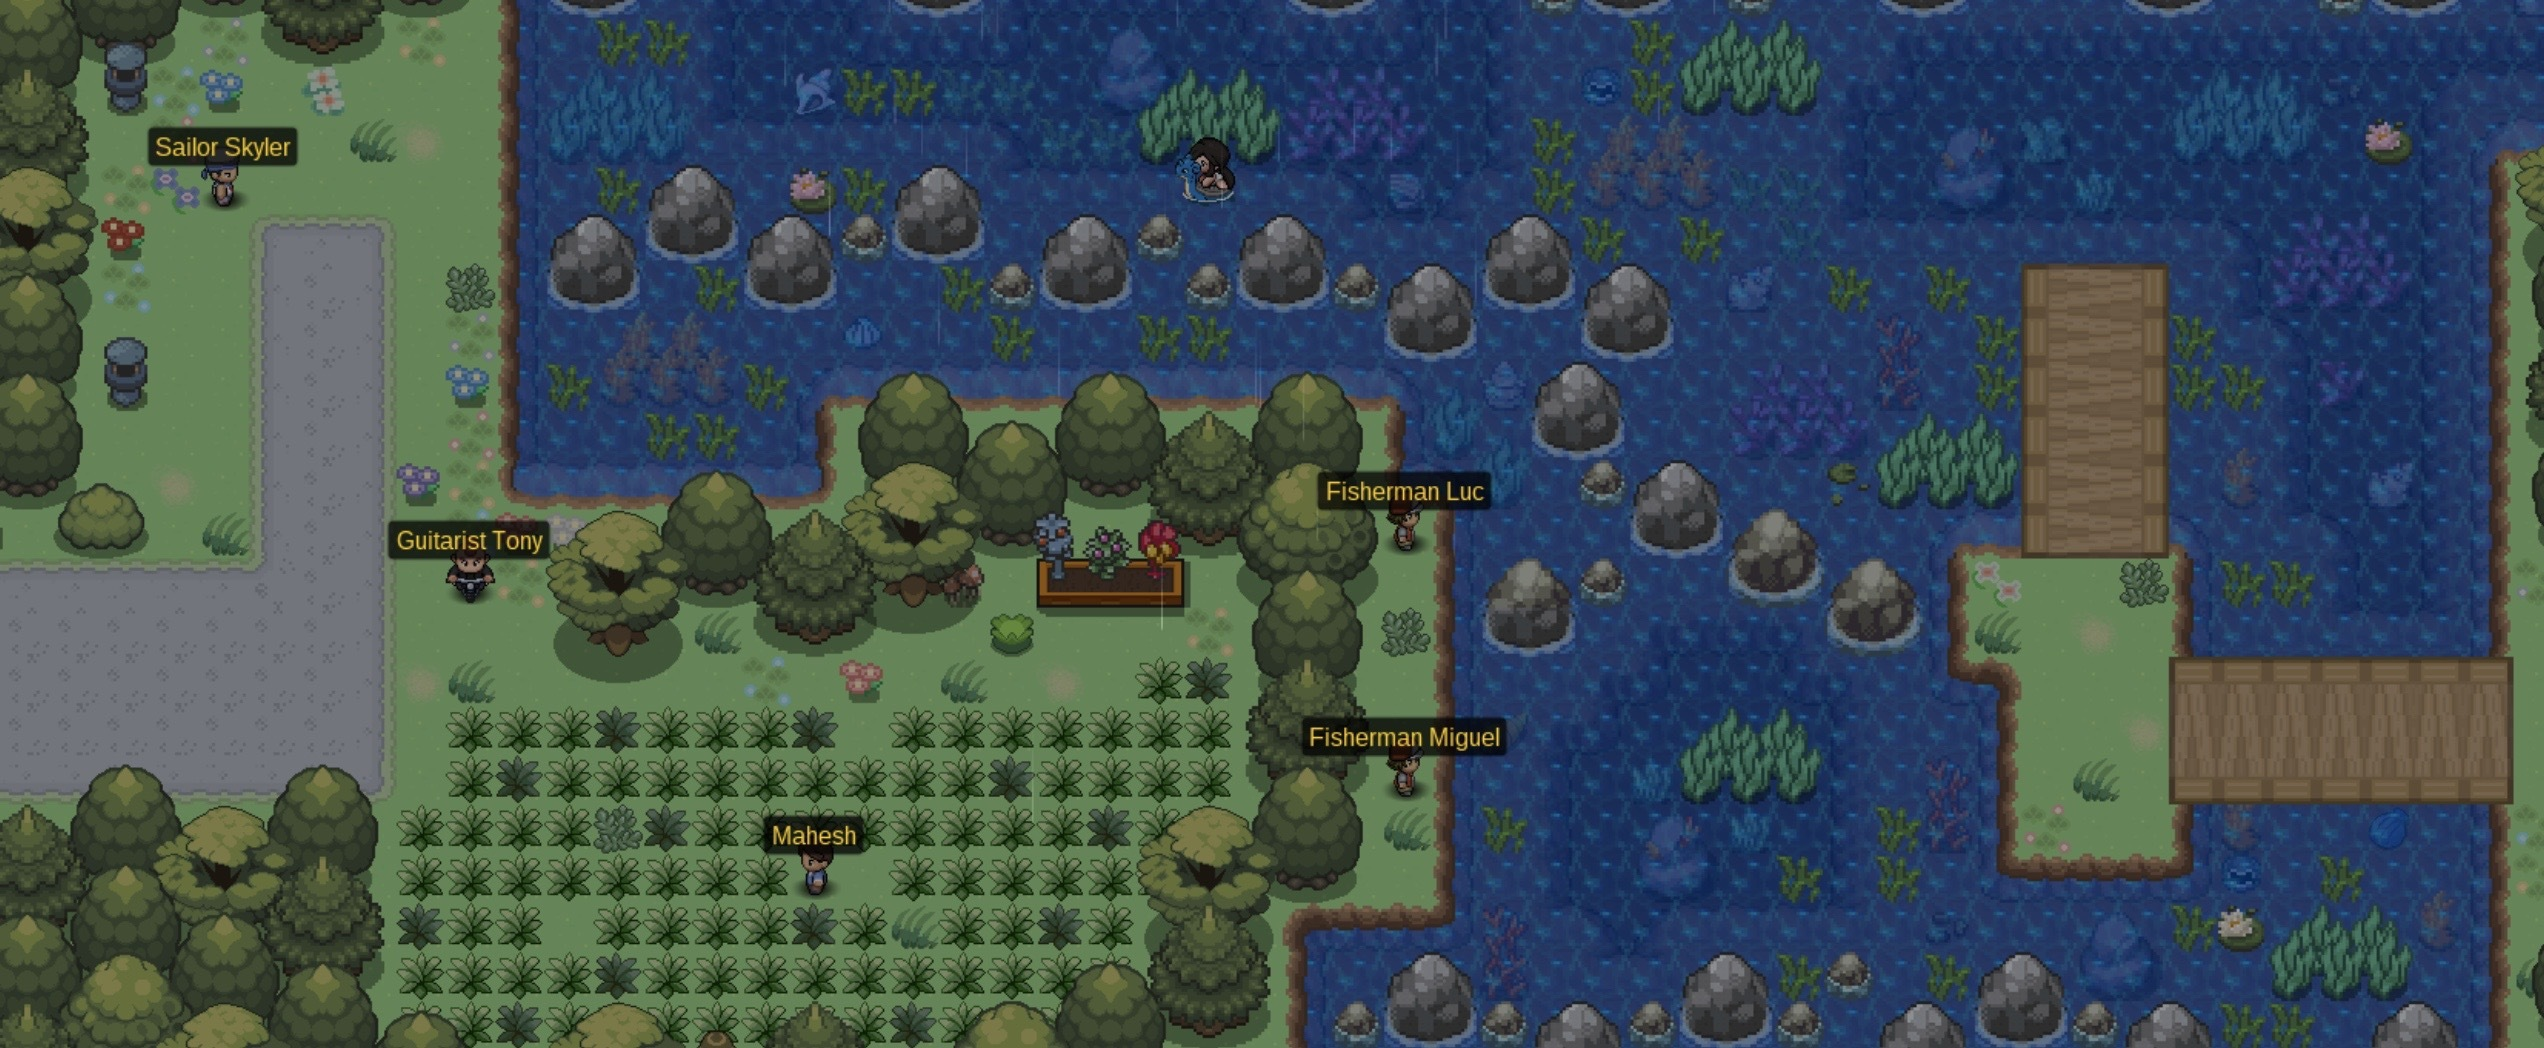
\includegraphics[width=\textwidth]{walkthrough/Sinnoh/Route_218}

\paragraph{Route 218}
Backtrack to Jubilife.
Go west to Route 218.
Surf to the top right to get a Rare Candy.
Then, head west.

\input{routes/Sinnoh/Route_218/Wild_Pokémon_(Water)}

\section{Canalave City}\label{sec:canalave-city}
And finally we are in Canalave city.
Go to the gym and we are going to find barry blocking the way.
Talk with him and be ready to battle.
And now go to the gym.
This gym puzzle its easy so this time we dont need a tutorial.
Battle with trainers and beat the leader.
Byron uses Steel-type Pokemon.
Beat him and you will get the Mine badge.
He will tell us that we need to go to Snowpoint but first,
we are confronted by Barry again.

\section{Iron Island}\label{sec:iron-island}
There is no PokeCenter on Iron Island so bring healing items or Escape Ropes to save time.

Iron Island is an island off the northwestern coast of Sinnoh.
It was once a prosperous ore mine, but was shut down after the ore reserves dried up.
Since then, it was kept open as a training area and habitat for wild Pokémon.

% \input{routes/Sinnoh/Iron_Island/Wild_Pokémon_(Iron_Island)}

\paragraph{1F}
Go down the right ladder first.

\input{routes/Sinnoh/Iron_Island/Wild_Pokémon_(Iron_Island_1F)}

\paragraph{B1F}
Go down the right ladder first.

\input{routes/Sinnoh/Iron_Island/Wild_Pokémon_(Iron_Island_B1F_L)}
\input{routes/Sinnoh/Iron_Island/Wild_Pokémon_(Iron_Island_B1F_R)}

\paragraph{B2F}
On the right side, it's just a bunch of trainers.
On the left side, you can navigate to the entrance to the Exit Room.

\input{routes/Sinnoh/Iron_Island/Wild_Pokémon_(Iron_Island_B2F_L)}
\input{routes/Sinnoh/Iron_Island/Wild_Pokémon_(Iron_Island_B2F_R)}

\paragraph{Exit Room}
You can get TM Smart Strike here.

\input{routes/Sinnoh/Iron_Island/Wild_Pokémon_(Iron_Island_Exit_Room)}

\section{Prof Rowan and Trio Lakes}\label{sec:prof-rowan-and-trio-lakes}
Go to the library in Canalave City and go to the second floor.
There we are going to find Prof Rowan with Dawn and Barry,
we need to help him to protect the Guardians.

\subsection{Lake Valor}\label{subsec:lake-valor}
Now go back to Pastoria City and go to Valor Lakefront.
Get ready to battle with a lot of members of Team Galatic.
Go to the Cave and beat Saturn.

\input{routes/Sinnoh/Lake_Valor/Wild_Pokémon_(Land)}
\input{routes/Sinnoh/Lake_Valor/Wild_Pokémon_(Water)}
\input{routes/Sinnoh/Lake_Valor/Wild_Pokémon_(Headbuttable_Trees)}

\subsection{Lake Verity}\label{subsec:lake-verity}
After beating Saturn we need to go and help Prof Rowan and Dawn in Lake Verity, Go back to Route 201 and go to the left.
Battle with Mars and beat him

\subsection{Mt. Coronet North}\label{subsec:mt.-coronet-north}
And finally we need to help Barry in Lake Acuity.
To get there we must go back to Eterna City and to the right, into Mt. Coronet Center.
Go up, then into the basement, then further up into Mt. Coronet North.
Eventually you will find an exit to Route 216.

\input{routes/Sinnoh/Mt._Coronet_North/Wild_Pokémon_(Mt._Coronet_North)}

\subsection{Route 216}\label{subsec:route-2162}
Now we are in Route 216, nothing important in this route just a lot of trainers.

\input{routes/Sinnoh/Route_216/Wild_Pokémon_(Land)}

\section{Route 217}\label{sec:route-217}
Same as Route 216, In route 217 We are going to find a lot of trainers

\input{routes/Sinnoh/Route_217/Wild_Pokémon_(Land)}


\section{Acuity Lakefront}
But at the north we are going to find This Team Galactic blocking the way.
We need to get the Icicle Badge first.
Go to the right and We are in Snowpoint City.

\input{routes/Sinnoh/Acuity_Lakefront/Wild_Pokémon_(Land)}

\section{Snowpoint City}\label{sec:snowpoint-city}

\section{Lake Acuity}\label{sec:lake-acuity}
Go back to Acuity Lakefront and now Lake Acuity is accessible.
Talk with Barry, He will tell us that
he lost and we need to go to Team Galactic HQ in Veilstone City!

\section{Team Galactic Headquarters}\label{sec:team-galactic-headquarters}
Go back to Veilstone City and Talk with the guy in front of the HQ,
Beat him and he will give us the password!
Now go to the left of the city and enter this warehouse!
Use the password and go downstairs.
Follow the way until this room and take the Teleport!

\includegraphics[width=\textwidth]{walkthrough/Sinnoh/galactic-1}

Now follow the way again until this bin, Search in the bin and you will
find a paper with the pasword to open the next doors!

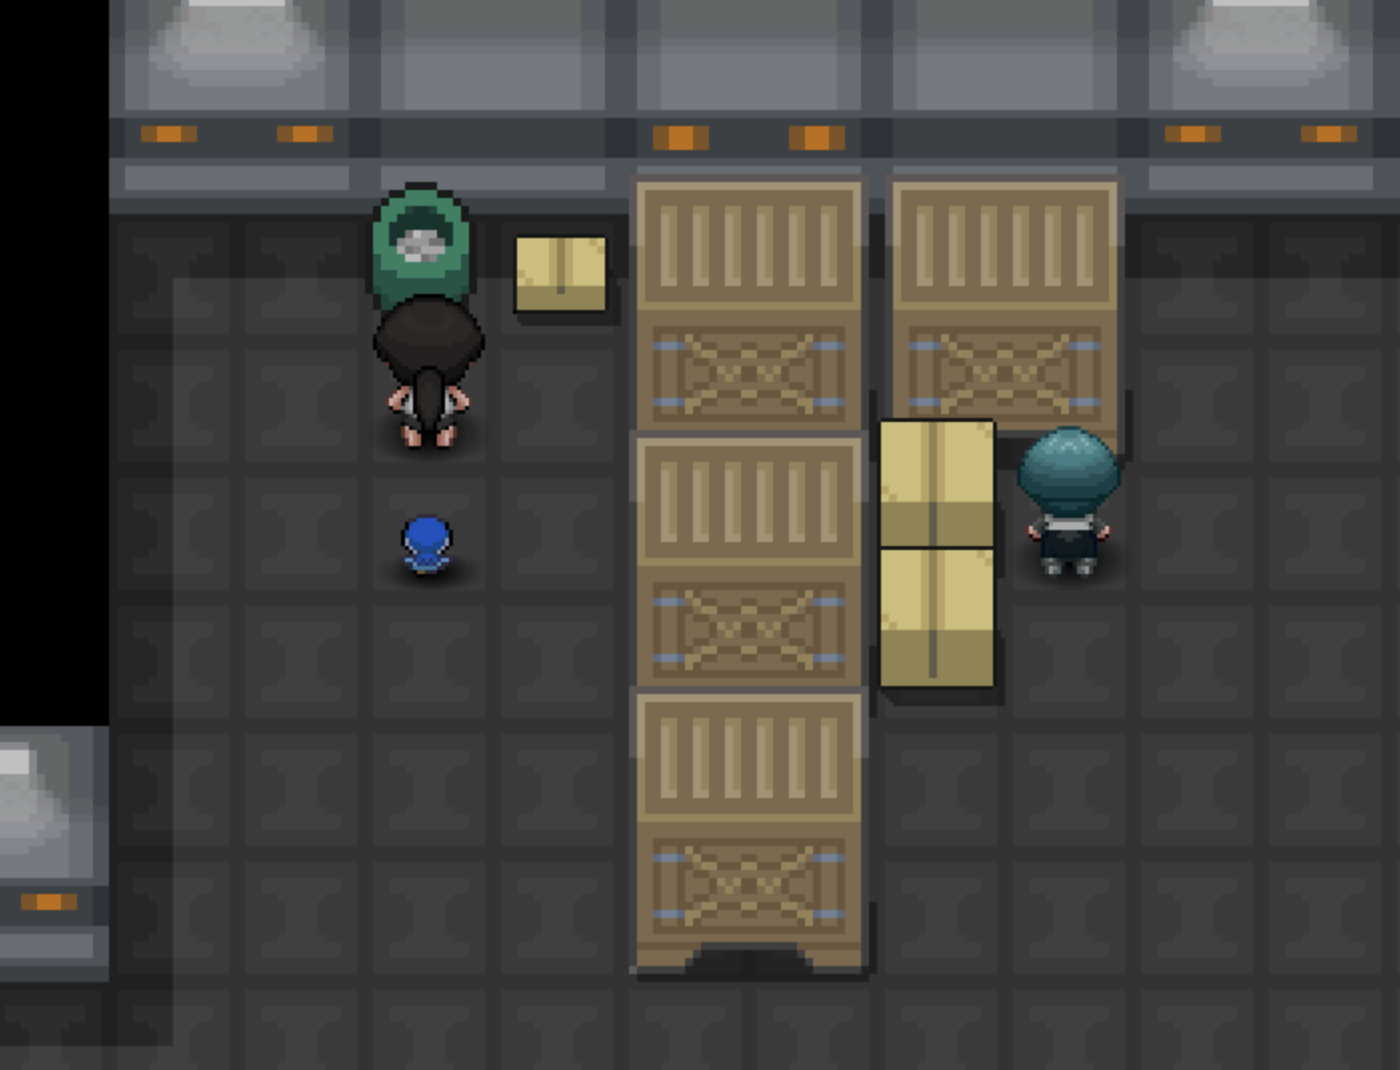
\includegraphics[width=\textwidth]{walkthrough/Sinnoh/galactic-2}

Now go back to the HQ and use the password to go up stairs!
Follow the way and use the teleporter in the room with a TV!

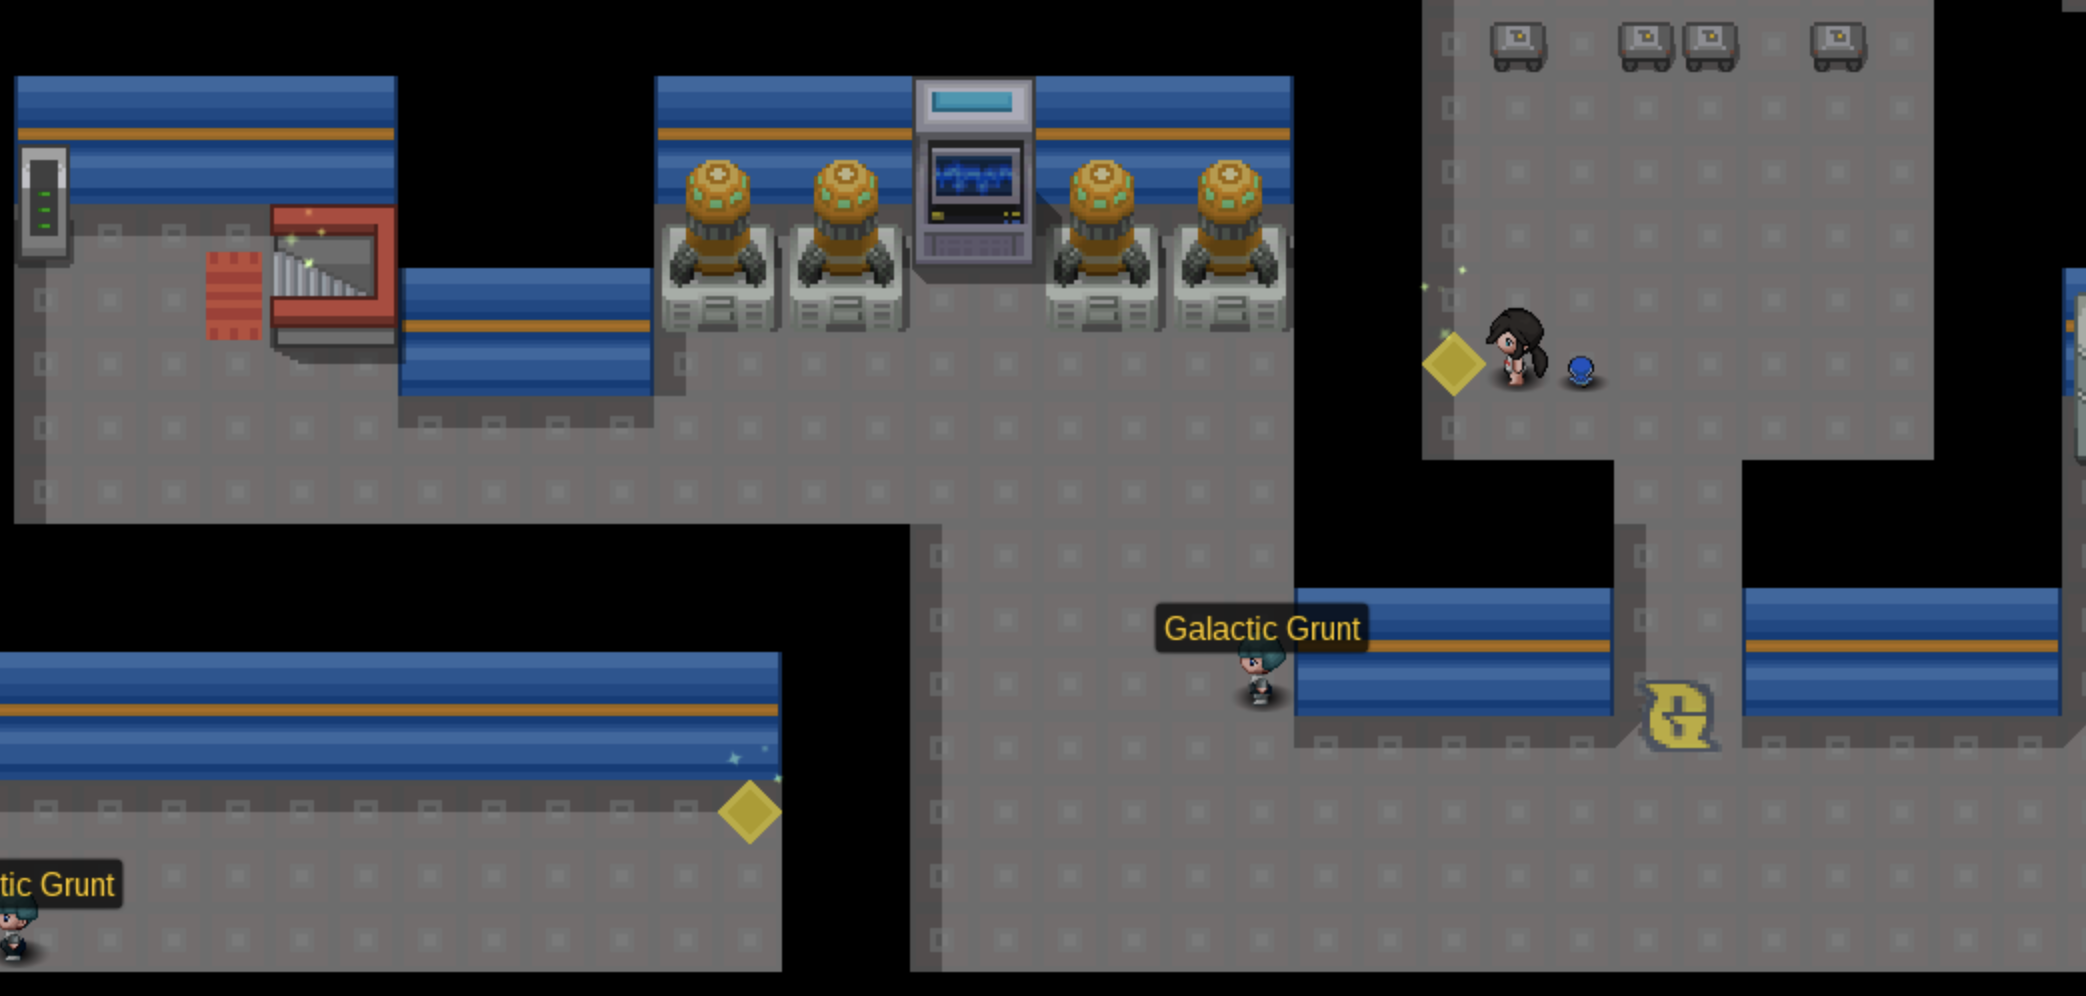
\includegraphics[width=\textwidth]{walkthrough/Sinnoh/galactic-3}

Now use the teleporter in the left!

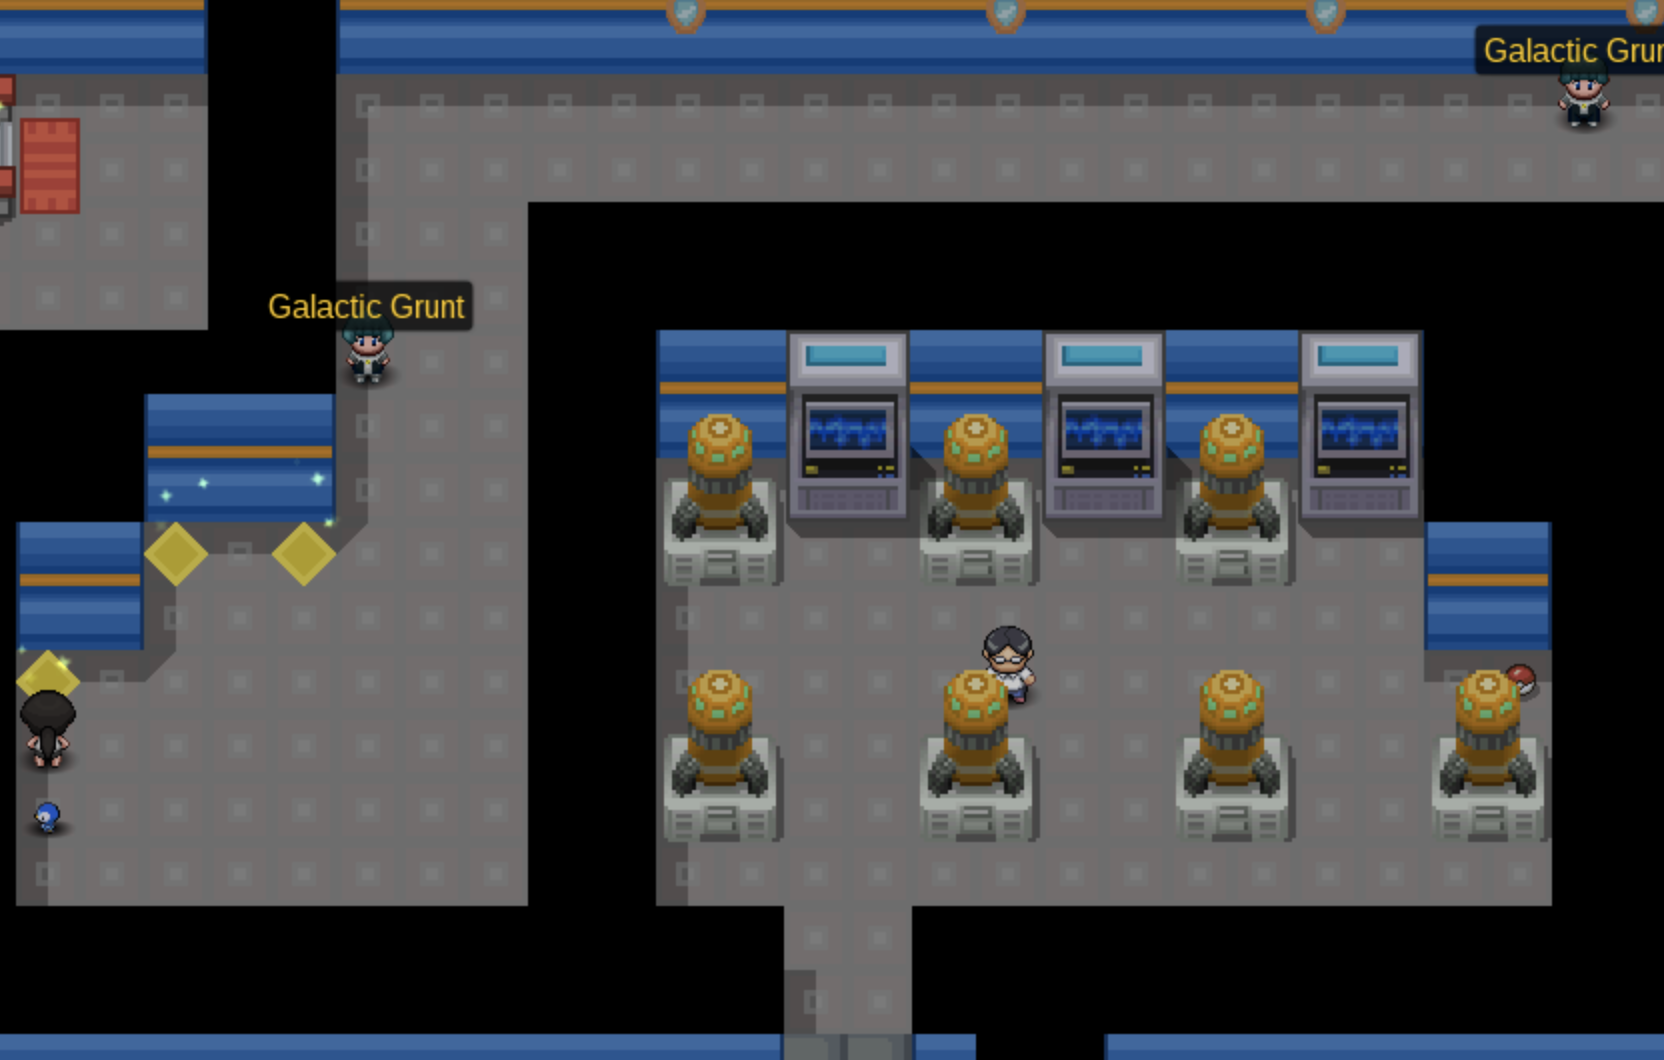
\includegraphics[width=\textwidth]{walkthrough/Sinnoh/galactic-4}

And finaly you will find Cyrus, Beat him!
After you beat him take the teleporter in the right!
And now be ready to battle with Saturn!
Beat him and now press the button in the machine!

\section{Back to Mt. Coronet}\label{sec:back-to-mt.-coronet}
Now go back to Celestic Town and enter Mt. Coronet but this time go down!
Go to the top of the mountain and be ready for a lot of battles!
And finally we are in the top!, Talk with Cyrus and he will be
teleported to other dimension with Giratina!

\section{Distortion World}\label{sec:distortion-world}
Now get ready to go to Distortion World!
Now we are in the distortion world, 
follow the way until you find Cyrus and be ready to battle!
Once you beat him talk with Giratina and you need to beat him too!
Beat him and you will be teleported back with cynthia!

\section{Sendoff Spring}\label{sec:sendoff-spring}
Cynthia will offer to help you by teleporting to Route 214.
You can return to Sendoff Spring once you have healed your Pokemon.

\input{Routes/Sinnoh/Sendoff_Spring/Wild_Pokémon_(Land)}
\input{Routes/Sinnoh/Sendoff_Spring/Wild_Pokémon_(Water)}
\input{Routes/Sinnoh/Sendoff_Spring/Wild_Pokémon_(Headbuttable_Trees)}

\section{Route 222}\label{sec:route-222}
Go down and go to Route 222!
Nothing much in this route just a lot of trainers!

\input{routes/Sinnoh/Route_222/Wild_Pokémon_(Land)}
\input{routes/Sinnoh/Route_222/Wild_Pokémon_(Water)}

\section{Sunyshore City}\label{sec:sunyshore-city}

\section{Route 223}\label{sec:route-223}
Now get ready to E4, Go to route 223 and battle with a lot of trainers!
Now use Waterfall and enter Victory Road!

\input{routes/Sinnoh/Route_223/Wild_Pokémon_(Water)}

\section{Sinnoh Victory Road}\label{sec:sinnoh-victory-road}

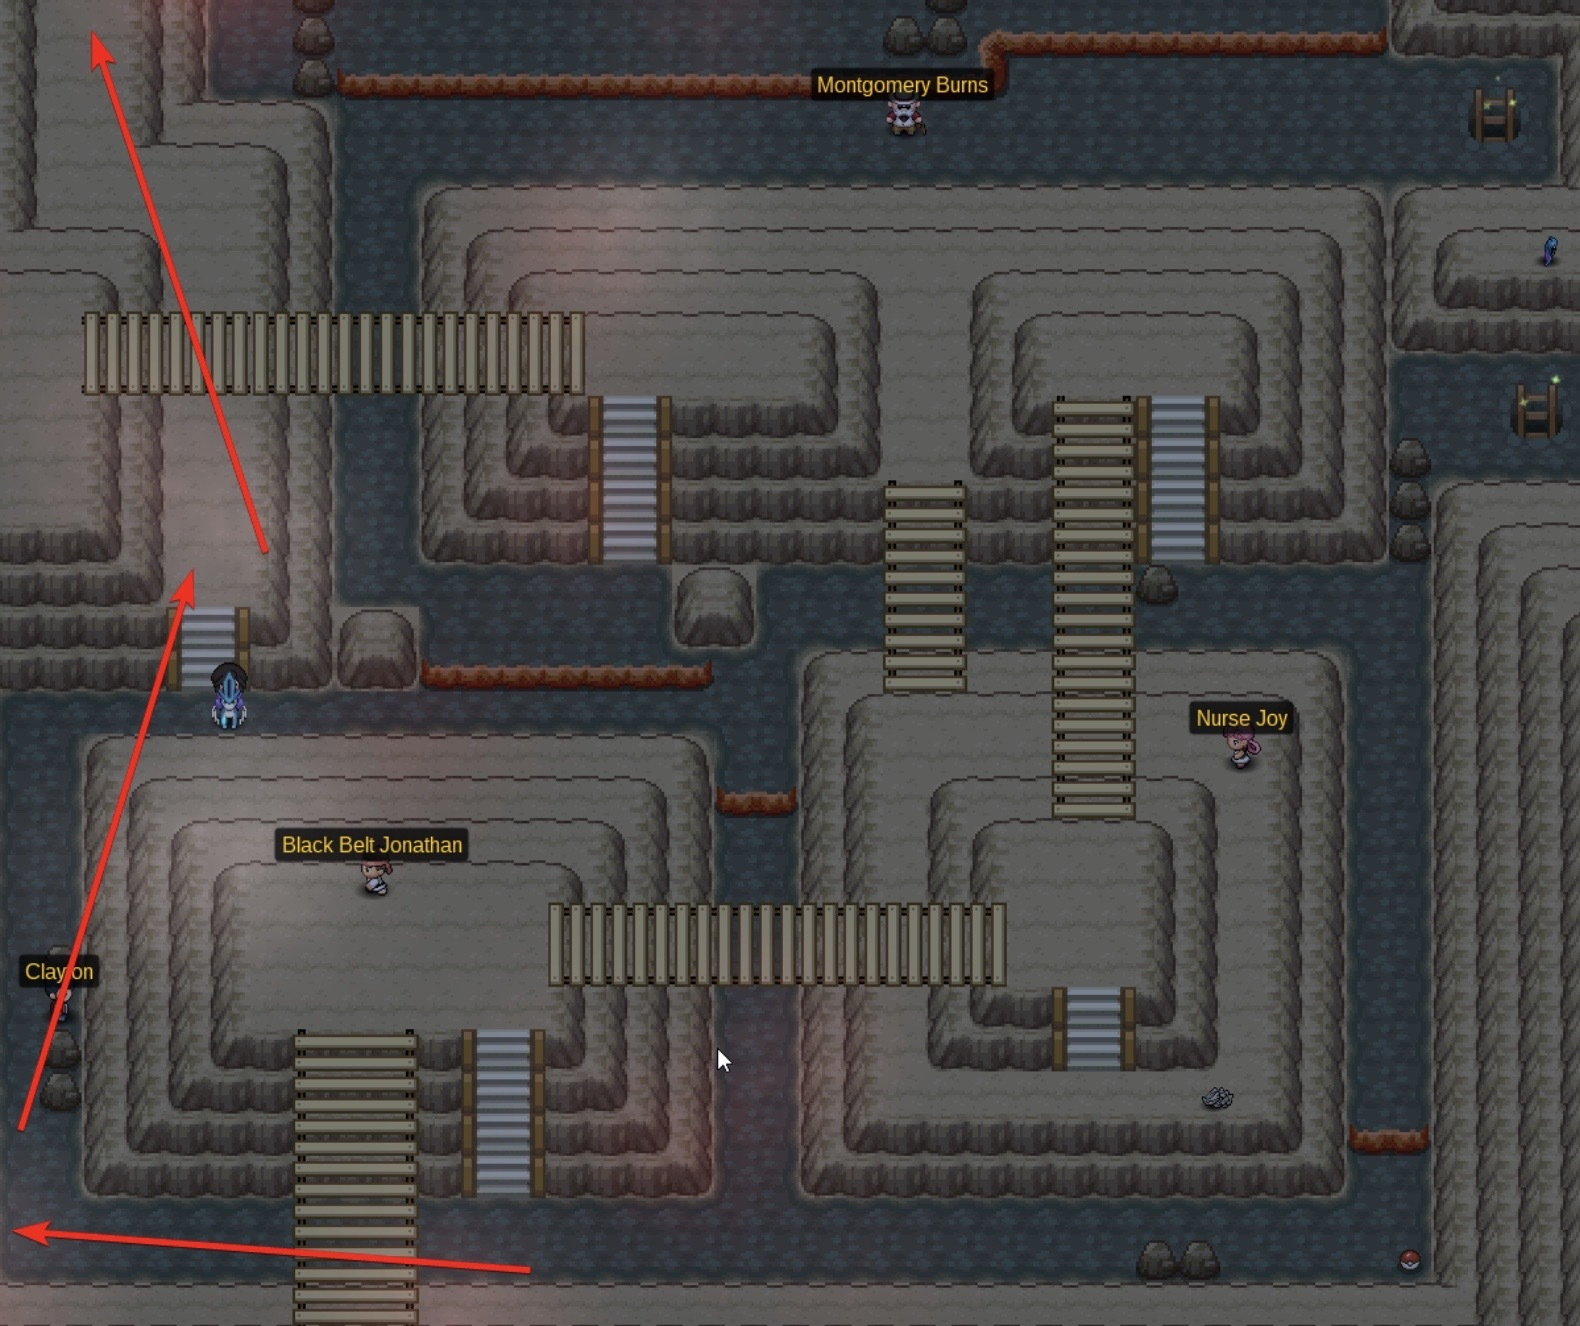
\includegraphics[width=\textwidth]{walkthrough/Sinnoh/victory-road-1}

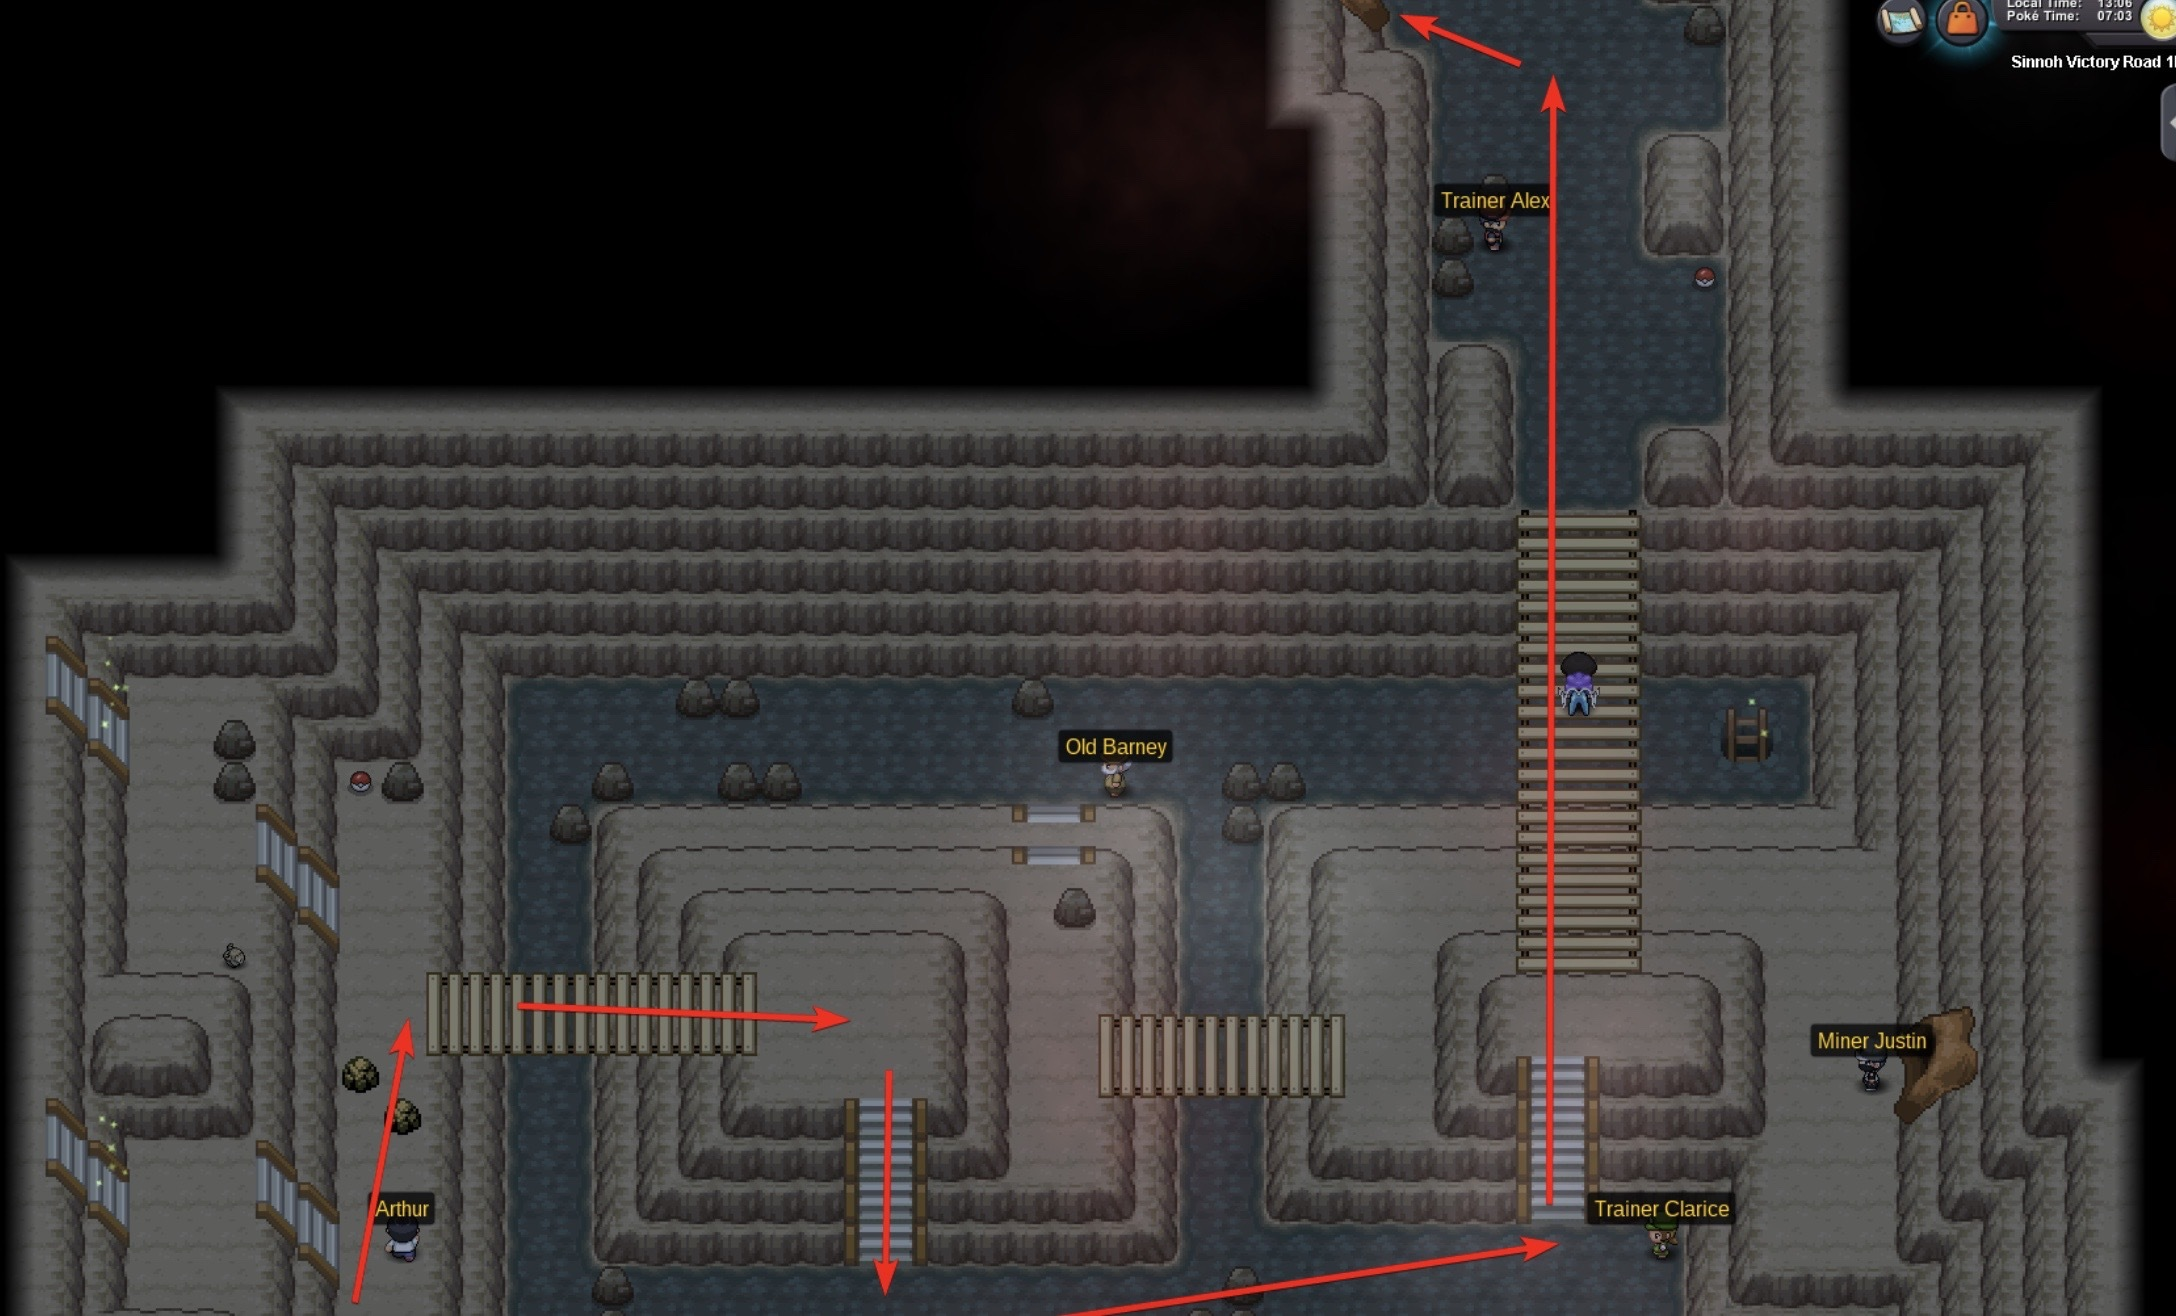
\includegraphics[width=\textwidth]{walkthrough/Sinnoh/victory-road-2}

\input{routes/Sinnoh/Sinnoh_Victory_Road_1F/Wild_Pokémon_(Sinnoh_Victory_Road_1F)}
\input{routes/Sinnoh/Sinnoh_Victory_Road_1F/Wild_Pokémon_(Sinnoh_Victory_Road_2F)}
% \input{routes/Sinnoh/Sinnoh_Victory_Road_1F/Wild_Pokémon_(Sinnoh_Victory_Road_B1F)}
% \input{routes/Sinnoh/Sinnoh_Victory_Road_1F/Wild_Pokémon_(Sinnoh_Victory_Road_B1F_Deep)}
\input{routes/Sinnoh/Sinnoh_Victory_Road_1F/Wild_Pokémon_(Sinnoh_Victory_Road_B1F_Deep_Entrance)}
\input{routes/Sinnoh/Sinnoh_Victory_Road_1F/Wild_Pokémon_(Sinnoh_Victory_Road_B1F_Deep_Exit)}

\thispagestyle{empty}
\listoffigures
\listoftables
\newpage
\pagenumbering{arabic}

\end{document}
